%-------------------------------------------------------------------------------
% Main file of presentation
%-------------------------------------------------------------------------------

\documentclass[t]{beamer}

%-------------------------------------------------------------------------------
% pdfLaTeX (not used)
%\usepackage[T1]{fontenc}
%\usepackage[utf8]{inputenc}
%\usepackage[american]{babel} %[ngerman]


%-------------------------------------------------------------------------------
% XeLaTeX (used)
\usepackage{polyglossia} % replaces babel
%\setmainlanguage[spelling=new,babelshorthands=true]{german}
%\usepackage{fontspec}
%\usepackage{relsize}
%\usepackage{microtype} % better management of overfulls

%-------------------------------------------------------------------------------
% beamer presentation theme (local to this project)
%\usetheme{beamerthemefau-4-3}
\usepackage{beamertheme/beamerthemefau-4-3}

%-------------------------------------------------------------------------------
% Quotes
%\usepackage[babel=once,german=quotes]{csquotes}

%-------------------------------------------------------------------------------
% strike out text with \st{some text}
\usepackage{soul}

%-------------------------------------------------------------------------------
% Images, captions
\usepackage{graphicx}
%\usepackage{subfig}
\usepackage{wrapfig}
\usepackage{caption}
\usepackage{subcaption}
%\DeclareCaptionFont{mysize}{\fontsize{14}{9.6}\selectfont}
%\captionsetup[sub]{font=mysize,labelfont={bf,sf}}
%\captionsetup{font=mysize,labelfont={bf,sf}}

%-------------------------------------------------------------------------------
% non-floating float environment, figure H option
\usepackage{float}
\usepackage{scrhack}

%-------------------------------------------------------------------------------
% Include text in graphics
\usepackage{psfrag}

%-------------------------------------------------------------------------------
% math, symbols, math font, units
\usepackage{amsmath}
\usepackage{amsbsy}
\usepackage{amssymb}
\usepackage{xfrac}
\usepackage{bm}
\usepackage{cancel}
\usepackage{commath} % provides differential operators
\usepackage{textcomp} % required by gensymb
\usepackage{gensymb} % eg. \degree symbol
\usepackage{mathtools} % eg. \underbrace

\usepackage[math-style=ISO]{unicode-math} % font (XeLaTeX)
%\usepackage{upgreek} % (non-italic print) greek letters

\usepackage{custom_math} % local to this project
\usepackage{units} % local to this project

%-------------------------------------------------------------------------------
% line break in citations
\usepackage{breakcites}

%-------------------------------------------------------------------------------
% colored and shaded boxes
\usepackage{color}
\usepackage{framed}

%-------------------------------------------------------------------------------
% theorem environment
\usepackage{theorem}

%-------------------------------------------------------------------------------
% tables with page break or flexible columns/rows
\usepackage{tabu}
\usepackage{longtable} % für Tabellen mit Seitenumbruch
\usepackage{multirow}
\usepackage{multicol}
\usepackage{makecell}
\usepackage{booktabs}
\usepackage{tabularx}

%-------------------------------------------------------------------------------
% make labels visible
%\usepackage{showkeys}

%-------------------------------------------------------------------------------
% links
\usepackage{hyperref}

%-------------------------------------------------------------------------------
% enumerate, itemize spacing
\usepackage{enumitem}
\setlist{  
  listparindent=\parindent,
  parsep=3pt, % space above each item
  topsep=2pt, % space above (all items together)
}
\setlist[itemize,1]{label=$\circ$}

% fix compatibility with beamer
\setitemize{label=\protect\usebeamerfont{itemize item}
                  \protect\usebeamercolor[fg]{itemize item}}
\setenumerate[1]{label=\protect\usebeamerfont{enumerate item}
                       \protect\usebeamercolor[fg]{enumerate item}
                       \insertenumlabel.}


%-------------------------------------------------------------------------------
% custom hyphenation
% e.g. write Neumann\hyp{}Randbedingung
\usepackage{hyphenat}


%-------------------------------------------------------------------------------
% code listings
% neither of these is working yet!!!

%\usepackage{verbatim} %simple option

%\usepackage{listings} %other (more advanced) option
%\definecolor{mygreen}{RGB}{28,172,0} % color values Red, Green, Blue
%\definecolor{mylilas}{RGB}{170,55,241}
%
%\lstset{language=Matlab,
%  %basicstyle=\color{red},
%  breaklines=true,
%  morekeywords={matlab2tikz},
%  keywordstyle=\color{blue},
%  morekeywords=[2]{1}, keywordstyle=[2]{\color{black}},
%  identifierstyle=\color{black},
%  stringstyle=\color{mylilas},
%  commentstyle=\color{mygreen},
%  showstringspaces=false,%without this there will be a symbol in the places where there is a space
%  numbers=left,
%  numberstyle={\tiny \color{black}},% size of the numbers
%  numbersep=9pt, % this defines how far the numbers are from the text
%  emph=[1]{for,end,break},emphstyle=[1]\color{red}, %some words to emphasize
%  %emph=[2]{word1,word2}, emphstyle=[2]{style},    
%}


%-------------------------------------------------------------------------------
% setup title page
\title[]{Elasticity of one-dimensional continua and nanostructures}
\author{Prof. Ajeet Kumar, Prakhar Gupta, Smriti Singh}
\date{Erlangen, Summer term 2017}
\institute{Chair of Applied Mechanics}

% TODO include IIT logo

%-------------------------------------------------------------------------------
% begin body of document and render title page

\begin{document}

% plain-option deactivates header and footer
\frame[plain,c]{\titlepage}



%-------------------------------------------------------------------------------
% include section introduction
%===============================================================================
\section*{Introduction}


%-------------------------------------------------------------------------------
\begin{frame}
  \frametitle{Extension, torsion and bending of rods/beams}
  
  \begin{tabularx}{\linewidth}{XX}
    {
    \begin{alignat*}{1}
      F &= E \, A \, \epsilon \\
        %&= E \, A \, \frac{\Delta l}{l}
    \end{alignat*}
    } & {
    \null
    } \\
    %\hline
    
    {
    \begin{alignat*}{1}
      M_t = G \, J \, \frac{\Theta}{L} \\
    \end{alignat*}
    } & {
    \null
    } \\
    %\hline
        
    {
    \begin{alignat*}{1}
      M = E \, I \, \kappa \\
    \end{alignat*}
    } & {
    \null
    }
  \end{tabularx}  
  
  % TODO revisit this/these motivational slide/slides
  % put in three pictures
\end{frame}


%-------------------------------------------------------------------------------
\begin{frame}
  \frametitle{3D elasticity (recap of some basics)}
  
  \textbf{deformation map} $\underline{x} = \underline{f}(\underline{X})$
  \begin{itemize}
    \item takes a (Langrangian/material) vector/point $\underline{X}$ in the undeformed configuration
    \item returns a (Eulerian/spatial) vector/point $\underline{x}$ in the deformed configuration
  \end{itemize}
  \vspace{1em}
  
  \textbf{deformation gradient} $\doubleunderline{F}(\underline{X}) = \nabla_{\underline{X}} \,\underline{f}(\underline{X})$
  \begin{itemize}
    \item takes a (Langrangian/material) vector/point $\underline{X}$ in the undeformed configuration \newline
      $\rightarrow$ $\underline{X}$ is material point where the gradient is evaluated
    \item returns a second order (two-point) tensor $\doubleunderline{F}$ that depends on $\underline{X}$ (in the general case)
    \item $\doubleunderline{F}$ contains (first order accurate) information about how line elements in the material configuration are transformed into deformed (stretched and rotated) line elements in the spatial configuration by $\underline{f}(.)$ \newline
      $\rightarrow$ $\dif \underline{x} = \doubleunderline{F}(\underline{X}) \cdot \dif \underline{X}= \nabla_{\underline{X}} \,\underline{f}(\underline{X}) \cdot \dif \underline{X}$
  \end{itemize}
  \vspace{1em}
  
  \textbf{equations of equilibrium}
  \begin{itemize}
    \item material description: $\nabla_{\underline{X}} \cdot \doubleunderline{P} + \underline{B} = \rho_0 \cdot \underline{A}$
    \item spatial description: $\nabla_{\underline{x}} \cdot \doubleunderline{\sigma} + \underline{b} = \rho \cdot \underline{a}$
  \end{itemize}
\end{frame}


%-------------------------------------------------------------------------------
\begin{frame}
  \frametitle{1D elasticity}
  
  we talk about \textbf{slender bodies} ($\frac{\mathrm{Length}}{\mathrm{Diameter}} > 10$)
  \vspace{1em}
  
  we only have \textbf{one material coordinate} $s$ along the axis of the beam
  \begin{itemize}
    \item $s$ uniquely identifies a particular cross section along the beam axis
    \item model equations will be a system of ODEs in $s$ (instead of PDE)
    \item equations are obtained by averaging a PDE in 3 dimensions over the cross section
  \end{itemize}
  \vspace{1em}
  
  kinematic quantities in the model
  \begin{itemize}
    \item \textbf{position of centerline} $\underline{r}(s)$
    \item \textbf{orientation/rotation of cross section} $\doubleunderline{R}(s)$
    \item more accuracy $\rightarrow$ more unknowns
  \end{itemize}
\end{frame}




%-------------------------------------------------------------------------------
% section content of the presentation, overview, table of contents
\section*{Outline of this course}

% render table of contents page
\frame{
  \tableofcontents
}


%-------------------------------------------------------------------------------
% include section traditional_beams
%===============================================================================
\section{Traditional beam models}

%===============================================================================
\subsection{Euler-Bernoulli beam theory}

%-------------------------------------------------------------------------------
\begin{frame}
  \frametitle{The Euler-Bernoulli beam (planar case)}
  
  \begin{itemize}
    \item assumption of the model
      \begin{itemize}
        \item all cross sections remain planar
        \item cross section normal and centerline tangent are of same orientation $\varphi$ \newline
          \null \quad $\rightarrow$ model only allows for pure bending (no shear)
      \end{itemize}
    \item bending moment $M(s) = E \, I \, \kappa(s)$
    \item centerline of beam described by function $y(s)$
    \item curvature of centerline given by $\kappa(s) = \frac{\od[2]{y}{s}(s)}{\biggl( 1 + \bigl( \od{y}{s}(s) \bigr)^2 \biggr)^{\frac{3}{2}}}$ \newline
      \null \quad $\rightarrow$ geometric nonlinearity $\rightarrow$ non-linear ODE
    \item linear approximation for small deflections: $\od{y}{s} = \tan(\varphi) \ll 1 \Rightarrow \od{y}{s} \approx \varphi$
    \item Euler-Bernoulli beam equation: $M(s) = E \, I \, \od[2]{y}{s}$
  \end{itemize}
\end{frame}


%-------------------------------------------------------------------------------
\begin{frame}
  \frametitle{Example: Cantilever beam (part 1)}
  
  \begin{figure}
    \centering
    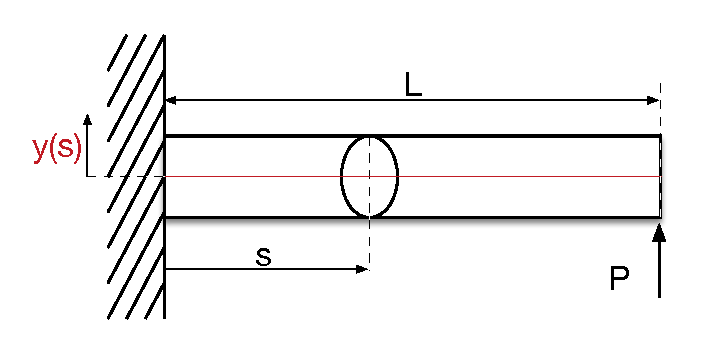
\includegraphics[width=16cm, keepaspectratio=true]{sections/traditional_beams/images/EulerCanitleverExample1part1}
  \end{figure}
  
  \begin{tabularx}{\linewidth}{XX}
    {
      boundary conditions at $s=0$:
      \begin{itemize}
        \item $y(0) = 0$
        \item $\od{y}{s}(0) = 0$
      \end{itemize}
    } & {
      boundary conditions at $s=L$:
      \begin{itemize}
        \item $v(L) = P$
        \item $M(L) = 0 \Rightarrow \od[2]{y}{s}(L) = 0$
      \end{itemize}
    }
  \end{tabularx}
\end{frame}

%-------------------------------------------------------------------------------
\begin{frame}
  \frametitle{Example: Cantilever beam (part 2)}
  
  \begin{figure}
    \centering
    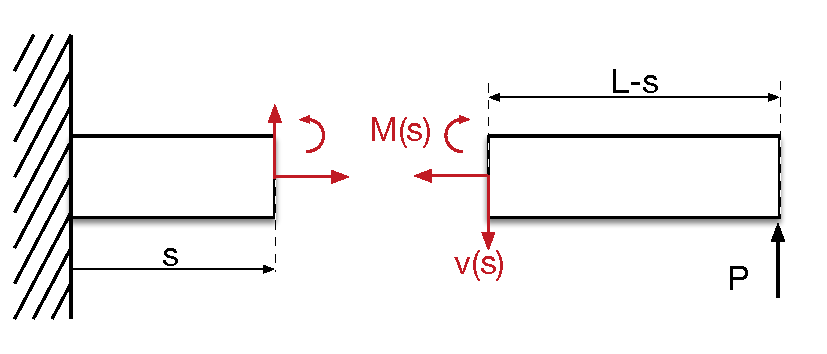
\includegraphics[width=14cm, keepaspectratio=true]{sections/traditional_beams/images/EulerCanitleverExample1part2}
  \end{figure} 
  \vspace{-1.4em}
  
  \begin{displaymath}
  \text{moment balance:} \quad  -M(s) + P(L-s) = 0 \quad \Rightarrow \quad M(s) = P \, (L-s)
  \end{displaymath}
  
  \begin{displaymath}
    M(x) = E \, I \, \od[2]{y}{s} \quad \Rightarrow \quad \od[2]{y}{s} = \frac{M(s)}{E \, I}  = \frac{P \, (L-s)}{E \, I}
  \end{displaymath}
  
  \begin{displaymath}
    \Rightarrow y(s) = \frac{P}{E \, I} \, \biggl( - \frac{s^3}{6} + \frac{L \, s^2}{2} \biggr) + \cancel{c_1} \,s + \cancel{c_2} = \frac{P \, L^3}{2 \, E \, I} \Biggl( \biggl( \frac{s}{L} \biggr)^2 - \frac{1}{3} \biggl( \frac{s}{L} \biggr)^3 \Biggr)
  \end{displaymath}
\end{frame}

%-------------------------------------------------------------------------------
\begin{frame}
  \frametitle{Another example of a cantilever beam}
  
  \begin{figure}
    \centering
    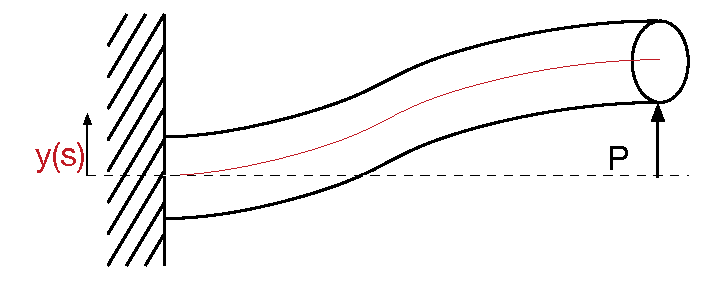
\includegraphics[width=16cm, keepaspectratio=true]{sections/traditional_beams/images/EulerCanitleverExample2}
  \end{figure}
  
  \begin{tabularx}{\linewidth}{XX}
    {
      boundary conditions at $s=0$:
      \begin{itemize}
        \item $y(0) = 0$
        \item $\od{y}{s}(0) = 0$
      \end{itemize}
    } & {
      boundary conditions at $s=L$:
      \begin{itemize}
        \item $v(L) = P$
        \item $\od{y}{s}(L) = 0 \Rightarrow M(L) \neq 0$ \newline
          \null \quad (rotation is restricted)
      \end{itemize}
    }
  \end{tabularx}
  
  \begin{displaymath}
    \Rightarrow M(s) = M(L) + P \, (L-s)
  \end{displaymath}
\end{frame}


%-------------------------------------------------------------------------------
\begin{frame}
  \frametitle{Boundary conditions}
  
  \vspace{4em}
  \begin{center}
    \begin{tabular}{lr}
      displacement & force \\
      \hline
      prescribed $\Rightarrow$ & unknown \\
      unknown & $\Leftarrow$ prescribed \\
      \hline \\
      \\
      rotation & moment \\
      \hline
      prescribed $\Rightarrow$ & unknown \\
      unknown & $\Leftarrow$ prescribed \\
      \hline
    \end{tabular}
  \end{center}
\end{frame}


%===============================================================================
\subsection{Timoshenko beam theory}


%-------------------------------------------------------------------------------
\begin{frame}
  \frametitle{The Timoshenko beam (planar case)}
  
  \vspace{-1em}
  \begin{figure}
    \centering
    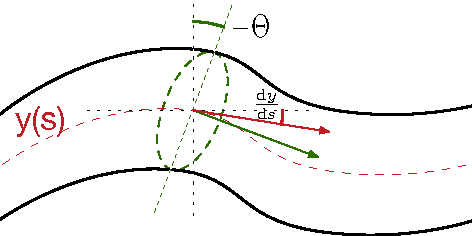
\includegraphics[width=16cm, keepaspectratio=true]{sections/traditional_beams/images/TimoshenkoBeam1}
  \end{figure}
  
  \begin{itemize}
    \item individual cross sections still remain planar
    \item centerline tangent orientation (red) $\neq$ cross section normal (green)
      \begin{itemize}
        \item $-\Theta$ measures orientation of cross section
        \item centerline tangent $\od{y}{s}$ influenced by \textbf{bending and shearing}
      \end{itemize}
    \item shear strain $\gamma(s) = \od{y}{s}(s) - \Theta(s) = \frac{v(s)}{k \, G \, A}$
    \item curvature $\kappa(s) = \od{\Theta}{s}(s) = \frac{M(s)}{E \, I}$ (see next slide)
  \end{itemize}
\end{frame}


%-------------------------------------------------------------------------------
\begin{frame}
  \frametitle{Connection between curvature and moment}

  \begin{multicols}{2}
    \noindent
    
    \begin{figure}
    \centering
      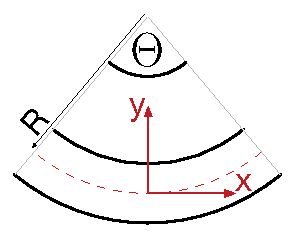
\includegraphics[width=13cm, keepaspectratio=true]{sections/traditional_beams/images/TimoshenkoBeam2}
    \end{figure}
    
    \begin{displaymath}
      L = R \, \Theta \quad \Rightarrow \quad \frac{1}{R} = \frac{\Theta}{L} = \od{\Theta}{s}
    \end{displaymath}
    
    \vspace{0.5em}
    fitting circles to the centerline locally:
    \begin{displaymath}
      \kappa(s) = \od{\Theta}{s}(s)
    \end{displaymath}
    
    \begin{displaymath}
      \epsilon_{xx} = \frac{\Delta L}{L} = \frac{(R-y) \, \Theta - R \, \Theta}{R \, \Theta} = \frac{-y}{R}
    \end{displaymath}
    
    \begin{displaymath}
      \sigma_{xx} = -E \, \frac{y}{R}
    \end{displaymath}
    
    \begin{displaymath}
      M = - \int_{\Omega} y \, \sigma_{xx} \, \dif A = E \, I \, \frac{1}{R} = E \, I \, \kappa
    \end{displaymath}
  \end{multicols}
\end{frame}


%-------------------------------------------------------------------------------
\begin{frame}
  \frametitle{Bending and axial compression together}

  \begin{multicols}{2}
    \noindent
    
    \begin{figure}
    \centering
      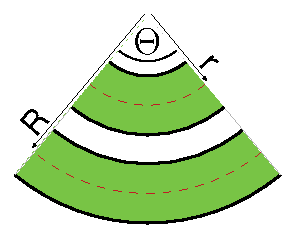
\includegraphics[width=13cm, keepaspectratio=true]{sections/traditional_beams/images/TimoshenkoBeam3}
    \end{figure}
      
    because of axial forces the beam got shorter!
    \begin{displaymath}
      \begin{alignedat}{1}
        \epsilon_{xx} &= \frac{(r-y) \, \Theta - R \, \Theta}{R \, \Theta} = \frac{r-R}{R} + \frac{-y}{R} \\ 
        &= \epsilon - \frac{y}{R}
      \end{alignedat}
    \end{displaymath}
    
    \vspace{0.2em}
    stress due to axial stretch + bending:
    \begin{displaymath}
      \sigma_{xx} = E \, \bigl( \epsilon + \frac{-y}{R} \bigr)
    \end{displaymath}
    
    \vspace{-0.7em}
    \begin{displaymath}
      \begin{alignedat}{1}
        M &= - \int_{\Omega} y \, \sigma_{xx} \, \dif A \\
          &= - E \, \epsilon \cancel{\int_{\Omega} y \, \dif A} + \frac{E}{R} \int_{\Omega} y^2 \dif A \\ 
          &= E \, I \, \kappa
      \end{alignedat}
    \end{displaymath}
    
    $\rightarrow$ bending and axial stretch are independent!
  \end{multicols}
\end{frame}


%-------------------------------------------------------------------------------
\begin{frame}
  \frametitle{Model linearity}
  
  \begin{displaymath}
    \begin{alignedat}{1}
      \od{y}{s} &= \frac{1}{k \, G \, A} \cdot v(s) + \Theta  \\ \\
      \od{\Theta}{s} &= \frac{1}{E \, I} \cdot M(s)
    \end{alignedat}
  \end{displaymath}

  \vspace{1em}
  we obtained a linear model because we assumed...
  \begin{itemize}
    \item small slopes of the centerline (linear kinematics)
      \begin{itemize}
        \item $\od{y}{s} = \tan{\Theta} \approx \Theta$
        \item approximation is not valid for larger deformations
      \end{itemize} 
    \item material linearity (linear constitutive law)
      \begin{itemize}
        \item $v(s)$, $M(s)$ get multiplied by constants \newline
          or by functions that depend on $s$ but not on $v(s)$, $M(s)$
        \item material may eg. get stiffer with increasing deformation energy
        \item btw. $k$ is a correction factor, that depends on the shape of the beam's cross section
      \end{itemize}
  \end{itemize}
\end{frame}

%-------------------------------------------------------------------------------
\begin{frame}
  \frametitle{Example: Cantilever beam (part 1)}
  
  \begin{figure}
    \centering
    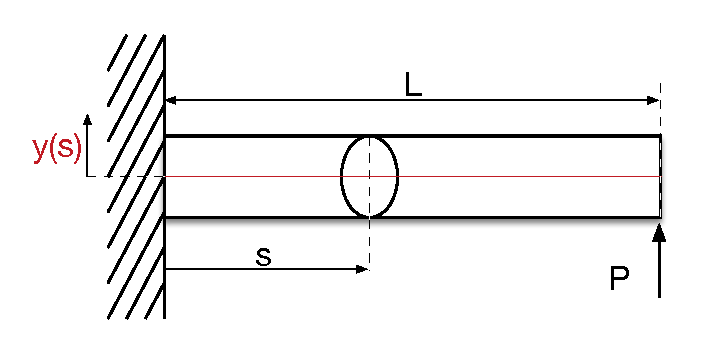
\includegraphics[width=16cm, keepaspectratio=true]{sections/traditional_beams/images/EulerCanitleverExample1part1}
  \end{figure}
  
  \begin{tabularx}{\linewidth}{XX}
    {
      boundary conditions at $s=0$:
      \begin{itemize}
        \item $y(0) = 0$
        \item $\xcancel{\od{y}{s}(0) = 0}$ (because of shear!)
        \item $\Theta(0) = 0$ (cross section fixed)
      \end{itemize}
    } & {
      boundary conditions at $s=L$:
      \begin{itemize}
        \item $v(L) = P$
        \item $M(L) = 0$
      \end{itemize}
    }
  \end{tabularx}
\end{frame}

%-------------------------------------------------------------------------------
\begin{frame}
  \frametitle{Example: Cantilever beam (part 2)}
  
  As before with the Euler-Bernoulli cantilever beam we have
  \begin{displaymath}
    v(s) = P \quad \text{ and } \quad M(s) = P \, (L-s)
  \end{displaymath}
  
  \vspace{1em}
  We integrate the Timoshenko beam equations ...
  \vspace{0.3em}
  \begin{displaymath}
    \od{\Theta}{s}(s) = \frac{M(s)}{E \, I} = \frac{P \, (L-s)}{E \, I}
    \quad \Rightarrow \quad
    \Theta(s) = \frac{P}{E \, I} \biggl( L \, s - \frac{s^2}{2} \biggr) + \cancel{c}
  \end{displaymath}
  
  \vspace{1em}
  
  \begin{displaymath}
    \od{y}{s}(s) = \frac{v(s)}{k \, G \, A} + \Theta(s) = \frac{P}{k \, G \, A} + \frac{P}{E \, I} \biggl( L \, s - \frac{s^2}{2} \biggr)
  \end{displaymath}
  
  \begin{displaymath}
    \Rightarrow y(s) = \frac{P \, s}{k \, G \, A} + \frac{P}{E \, I} \biggl( L \frac{s^2}{2} - \frac{s^3}{6} \biggr) + \cancel{c} = \frac{P \, s}{k \, G \, A} + \frac{P \, L^3}{2 \, E \, I} \Biggl( 
      \biggl( \frac{s}{L} \biggr)^2 - \frac{1}{3} \biggl( \frac{s}{L} \biggr)^3 \Biggr)
  \end{displaymath}
\end{frame}


%-------------------------------------------------------------------------------
\begin{frame}
  \frametitle{Comparison of Euler-Bernoulli and Timoshenko cantilever beams}
  
  \textbf{Euler-Bernoulli beam}
  \begin{displaymath}
    y^{(E)}(s) = \frac{P \, L^3}{2 \, E \, I} \Biggl( \biggl( \frac{s}{L} \biggr)^2 - \frac{1}{3} \biggl( \frac{s}{L} \biggr)^3 \Biggr)
    \Rightarrow y^{(E)}(L) = \frac{P \, L^3}{3 \, E \, I}
  \end{displaymath}
  
  \textbf{Timoshenko beam}
  \begin{displaymath}
    y^{(T)}(s) = \frac{P \, s}{k \, G \, A} + \frac{P \, L^3}{2 \, E \, I} \Biggl( 
      \biggl( \frac{s}{L} \biggr)^2 - \frac{1}{3} \biggl( \frac{s}{L} \biggr)^3 \Biggr)
      \Rightarrow y^{(T)}(L) = \frac{P \, L}{k \, G \, A} + \frac{P \, L^3}{3 \, E \, I}
  \end{displaymath}
  
  \textbf{relative error} (taking Euler-Bernoulli as the reference)
  \begin{displaymath}
    \begin{alignedat}{1}
      \epsilon_r &= \frac{y^{(T)}(L) - y^{(E)}(L)}{y^{(E)}(L)} = \frac{\frac{P \, L}{k \, G \, A}}{\frac{P \, L^3}{3 \, E \, I}} = \frac{3 \, E \, I}{k \, G \, A \, L^2} \\
      &= \frac{3 \, E \, b \, h^3}{k \, G \, b \, h \, L^2 \, 12} = \frac{1}{4} \frac{E}{k \, G} \biggl( \frac{h}{L} \biggr)^2
    \end{alignedat}
  \end{displaymath}
  
  \begin{center}
    $\rightarrow$ Euler-Bernoulli beam model performs equally good as the Timoshenko model \newline when the beam is very slender ($h/L$ small)
  \end{center}
\end{frame}


%-------------------------------------------------------------------------------
\begin{frame}
  \frametitle{Another example of a cantilever beam (part 1)}
  
  \vspace{-0.7em}
  \begin{figure}
    \centering
    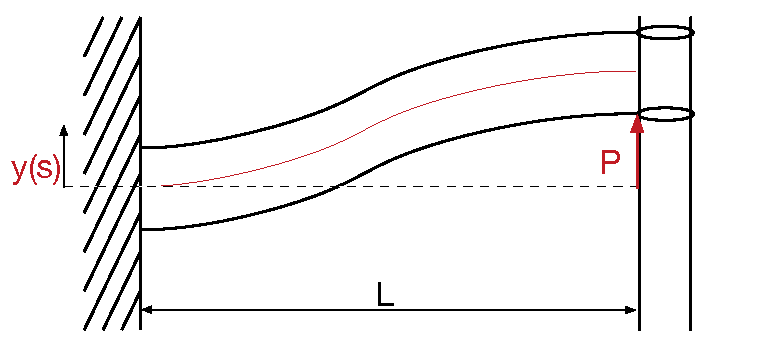
\includegraphics[width=16cm, keepaspectratio=true]{sections/traditional_beams/images/TimoshenkoCanitleverExample2part1}
  \end{figure}
  \vspace{-0.5em}
  cross section at $s=L$ can not rotate or displace horizontally
  \vspace{1em}
  \begin{tabularx}{\linewidth}{XX}
    {
      boundary conditions at $s=0$:
      \begin{itemize}
        \item $y(0) = 0$
        \item $\Theta(0) = 0$
      \end{itemize}
    } & {
      boundary conditions at $s=L$:
      \begin{itemize}
        \item $v(L) = P$
        \item $\Theta(L) = 0$
      \end{itemize}
    }
  \end{tabularx}
\end{frame}


%-------------------------------------------------------------------------------
\begin{frame}
  \frametitle{Another example of a cantilever beam (part 2)}
  
  \vspace{-0.7em}
  \begin{figure}
    \centering
    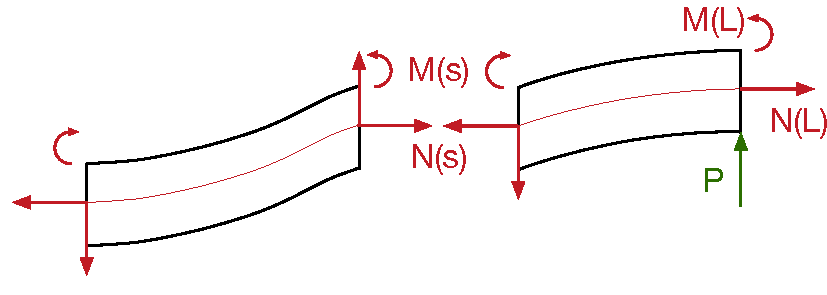
\includegraphics[width=20cm, keepaspectratio=true]{sections/traditional_beams/images/TimoshenkoCanitleverExample2part2}
  \end{figure}
  
  moment balance (in the deformed configuration):
  \begin{displaymath}
    -M(s) + M(L) + P \, (L-s) - N(y(L)-y(s))
  \end{displaymath}
  $\rightarrow$ the last term results in nonlinear behavior of the model \newline
  $\rightarrow$ $M(L)$ and $N(L)$ are two extra unknowns
\end{frame}


%-------------------------------------------------------------------------------
% include section cosserat_rods
%===============================================================================
\section{Theory of Special Cosserat rods}


%===============================================================================
\subsection{Kinematics of Cosserat rods}

%-------------------------------------------------------------------------------
\begin{frame}
  \frametitle{Introduction to \st{special} Cosserat rods (part 1)}
  
  \vspace{-1em}
  \begin{figure}
    \centering
    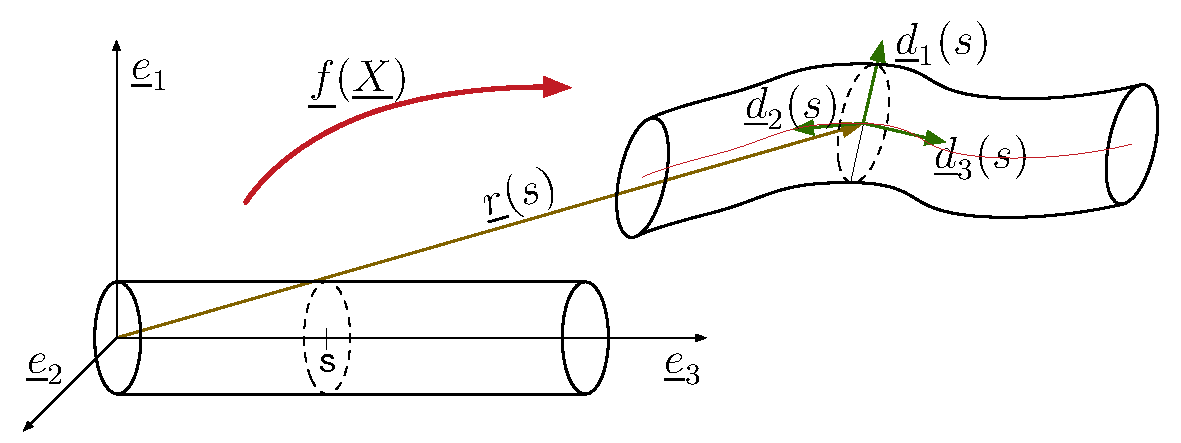
\includegraphics[width=20cm, keepaspectratio=true]{sections/cosserat_rods/images/Kinematics}
  \end{figure}
  
  remember: $s$ is the unique identifier for a particular cross section of the beam
  \vspace{0.6em}
  
  \textbf{kinematic quantities}:
  \begin{itemize}
    \item position of the deformed cross section $\underline{r}(s)$
    \item shearing of the deformed cross section $\underline{d}_1(s)$, $\underline{d}_2(s)$
    \item orientation of the deformed cross section $\underline{d}_3(s)$ \newline
      \null \quad (perpendicular to $\underline{d}_1(s)$ and $\underline{d}_2(s)$ $\rightarrow$ not independent)
    %\item $\doubleunderline{R}(s)$
  \end{itemize}
\end{frame}


%-------------------------------------------------------------------------------
\begin{frame}
  \frametitle{Introduction to \st{special} Cosserat rods (part 2)}

  \textbf{constrained deformation map}
  \begin{displaymath}
    \underline{f}(\underline{X}) = \underline{f}(X_1,X_2,X_3=s) = \underline{r}(s) + X_{\alpha} \, \underline{d}_{\alpha} \quad \text{with } \alpha \in \{1,2\}
  \end{displaymath}
  \vspace{1em}
  
  \textbf{consequences of the imposed kinematic constraints}
  \begin{itemize}
    \item cross sections remain flat
    \item straight lines within the cross section remain straight lines
    \item boundary of the cross section: circles are mapped to ellipses \newline
      \null \quad (not to arbitrary  curves in 2D)
    \item $\underline{d}_1(s)$ and $\underline{d}_2(s)$ are not perpendicular in the general case (shearing)
  \end{itemize}
\end{frame}


%===============================================================================
\subsection{Kinematics of Special Cosserat rods}


%-------------------------------------------------------------------------------
\begin{frame}
  \frametitle{What makes the Special Cosserat rod special?}

  \begin{itemize}
    \item $\underline{d}_1(s)$ and $\underline{d}_2(s)$ \textit{are} perpendicular and unit-normed
    \item hence $\left( \underline{d}_1, \underline{d}_2, \underline{d}_3 \right)$ form an orthonormal triad
  \end{itemize}
  \vspace{1em}
  
  \textbf{consequences}
  \begin{displaymath}
    \exists \: \doubleunderline{R}(s) \in SO(3) \: \forall s : \biggl( R: \left( \underline{e}_1, \underline{e}_2, \underline{e}_3 \right) \mapsto \left( \underline{d}_1, \underline{d}_2, \underline{d}_3 \right) \biggr)
  \end{displaymath}
  \begin{itemize}
    \item $\left( \underline{e}_1, \underline{e}_2, \underline{e}_3 \right)$ is called the global basis
    \item $\left( \underline{d}_1, \underline{d}_2, \underline{d}_3 \right)(s)$ is called the local basis or director basis at $s$
    \item $\underline{d}_i(s) = \doubleunderline{R}(s) \cdot \underline{e}_i$ \quad 
      ($\doubleunderline{R}$ : rotation matrix ; $SO(3)$ : special orthogonal matrix group)
  \end{itemize}
  \vspace{1em}
  
  \textbf{constrained deformation map}
  \begin{displaymath}
    \underline{f}(\underline{X}) = \underline{f}(X_1,X_2,X_3=s) = \underline{r}(s) + \doubleunderline{R}(s) \cdot (X_{\alpha} \, \underline{e}_{\alpha}) \quad \text{with } \alpha \in \{1,2\}
  \end{displaymath}
  
  \vspace{0.5em}
  $\rightarrow$ but the rigidity of the cross section is stiffening the beam!
\end{frame}


%-------------------------------------------------------------------------------
\begin{frame}
  \frametitle{Warp-mode on ;-)}
  
  we want to introduce warping of the cross section, \newline
  while at the same time keeping the director basis $\underline{d}_i$
  \vspace{0.6em}
  
  \textbf{modified deformation map}
  \begin{displaymath}
    \underline{f}(\underline{X}) = \underline{f}(X_1,X_2,X_3=s) = \underline{r}(s) + \doubleunderline{R}(s) \cdot (X_{\alpha} \, \underline{e}_{\alpha} + \underline{u}) \quad \text{with } \alpha \in \{1,2\}
  \end{displaymath}
  
  \vspace{0.3em}
  \textbf{geometric meaning of $\underline{u}$}
  \begin{itemize}
    \item $u_1$, $u_2$ : in-plane shrinking % TODO shrinking vs relative displacement
    \item $u_3$ : out-of-plane warping $\rightarrow$ cross section not planar anymore
    \item then $\underline{d}_1$, $\underline{d}_1$ represent the average orientation of the warped cross section
  \end{itemize}
  \vspace{0.6em}
  
  \textbf{what are our kinematic unknowns?}
  \begin{itemize}
    \item if $\underline{u} = \underline{u}(X_1,X_2,s)$ then we would be dealing with a 3D elasticity problem
    \item here we have $\underline{u}(X_1,X_2,\text{local strains})$, not a function of $s$ \newline (we will come back to this later)
    \item $\underline{r}(s)$ and $\doubleunderline{R}(s)$ are the only kinematic unknowns! (6 scalar quantities)
  \end{itemize}
\end{frame}


%-------------------------------------------------------------------------------
\begin{frame}
  \frametitle{Rotations in 3D revisited}
  
  a \textbf{rotation about \textit{one} axis} is determined by
  \begin{itemize}
    \item axis of rotation given by $\underline{a}$ with $\norm{\underline{a}} = 1$
    \item angle of rotation $\Theta$
  \end{itemize}
  \vspace{0.6em}
  
  \textbf{composition of rotations}
  \begin{displaymath}
    \left( \underline{a}_1, \Theta_1 \right) + \left( \underline{a}_2, \Theta_2 \right) + \left( \underline{a}_3, \Theta_3 \right) + \dots = \left( \underline{a}_{eff}, \Theta_{eff} \right)
  \end{displaymath}
  note: ``$+$'' here denotes the composition of two rotations
  
  \begin{displaymath}
    \doubleunderline{R}_{eff} = \dots \cdot \doubleunderline{R}_3 \cdot \doubleunderline{R}_2 \cdot \doubleunderline{R}_1
  \end{displaymath}
  
  In the general case ($\underline{a}_i \neq \underline{a}_j \text{ for } i \neq j$) rotations do not commute!
  \vspace{1em}
  
  \textbf{example} (rotation about $\underline{e}_3$):
  \begin{displaymath}
    \Biggl( \underline{a} =
    \begin{bmatrix}
      0 \\ 0 \\ 1
    \end{bmatrix}, \Theta \Biggr) \quad \rightarrow \quad
    \doubleunderline{R} =
    \begin{bmatrix}
      +\cos(\Theta) & -\sin(\Theta) & 0 \\
      +\sin(\Theta) & +\cos(\Theta) & 0 \\
      0 & 0 & 1
    \end{bmatrix}
  \end{displaymath}
\end{frame}

%-------------------------------------------------------------------------------
\begin{frame}
  \frametitle{Axis-angle representation of rotations in 3D}
  
  from the axis-angle representation
  \begin{displaymath}
    \Biggl( \underline{a} =
    \begin{bmatrix}
      a_1 \\ a_2 \\ a_3
    \end{bmatrix}, \Theta \Biggr)
  \end{displaymath}
  we obtain the corresponding rotation matrix
  \begin{displaymath}
    \doubleunderline{R} = \exp(\Theta \cdot \doubleunderline{a})  
  \end{displaymath}
  with
  \begin{displaymath}
    \Theta \cdot \doubleunderline{a} = \Theta \cdot 
    \begin{bmatrix}
      0 & -a_3 & a_2 \\
      a_3 & 0 & -a_1 \\
      -a_2 & a_1 & 0
    \end{bmatrix}
  \end{displaymath}
  a skew-symmetric matrix obtained from the definition
  \begin{displaymath}
    \doubleunderline{a} = \doubleunderline{a} \cdot \doubleunderline{I} =
%     \underline{a} \times \doubleunderline{I} :=
    \begin{bmatrix}
      \underline{a} \times \underline{e}_1 & \underline{a} \times \underline{e}_2 & \underline{a} \times \underline{e}_3
    \end{bmatrix}
  \end{displaymath}
  \begin{displaymath}
    \Rightarrow \quad
    \doubleunderline{a} \cdot \underline{v} = \underline{a} \times \underline{v} \quad \forall \underline{v} \in \mathbb{R}^3
  \end{displaymath}
  
  \vspace{0.5em}
  observe the isomorphism between cross products and skew-symmetric matrices:
  \begin{displaymath}
    \underline{a} = \axial(\doubleunderline{a}) = \axial(\underline{a} \times \doubleunderline{I}) = \axial([\underline{a}]_{\times})
  \end{displaymath}
\end{frame}


%-------------------------------------------------------------------------------
\begin{frame}
  \frametitle{Axis-angle representation of rotations in 3D: Rodrigues' formula}
  
  \begin{displaymath}
    \doubleunderline{R} = \cos(\Theta) \, \doubleunderline{I} + \sin(\Theta) \, \doubleunderline{a} + (1-\cos(\Theta)) \, \underline{a} \otimes \underline{a}
  \end{displaymath}
 
  \vspace{1em}
  the Rodrigues' rotation formula allows us to compute the rotation matrix $\doubleunderline{R}$,\newline
  that corresponds to a given axis-angle representation $\left( \underline{a}, \Theta \right)$, \newline
  without actually computing the matrix exponential
  
  \vspace{1em}
  computing matrix exponentials (of non-diagonal matrices) is either expensive or not precise!
  
  \vspace{2em}
  \textbf{example}
  \begin{displaymath}
    \underline{v}_{\text{rotated}} = \doubleunderline{R} \, \underline{v} = \cos(\Theta) \, \underline{v} + \sin(\Theta) \underline{a} \times \underline{v} + (1-\cos(\Theta)) \, (\underline{a} \cdot \underline{v}) \,\underline{a}
  \end{displaymath}
  
%  \begin{displaymath}
%    \doubleunderline{R} = \exp([\underline{a}]_{\times}) = \doubleunderline{I} + \sin(\norm{\underline{a}}) \biggl( \frac{\underline{a}}{\norm{\underline{a}}} \biggr)
%  \end{displaymath}
\end{frame}


%-------------------------------------------------------------------------------
\begin{frame}
  \frametitle{3D rotations expressed by unit quaternions}
  
  Quaternions are a number system that extends the complex numbers. A quaternion consists of one real part and three independent imaginary parts. A unit quaternion is a quaternion of norm one and therefore has three independent components. \newline
  There exists an isomorphism between unit quaternions and rotation matrices:

  \begin{displaymath}
    \text{given }
    \underline{q} = \begin{bmatrix}
      q_0 \\ q_1 \\ q_2 \\ q_3
    \end{bmatrix} \quad \rightarrow \quad
    \doubleunderline{R}(\underline{q}) = 2 \cdot \begin{bmatrix}
      \frac{1}{2} - (q_2^2 + q_3^2) & q_1 \, q_2 - q_0 \, q_3 & q_1 \, q_3 + q_0 \, q_2 \\
      q_1 \, q_2 + q_0 \, q_3 & \frac{1}{2} - (q_1^2 + q_3^2) & q_2 \, q_3 - q_0 \, q_1 \\
      q_1 \, q_3 - q_0 \, q_2 & q_2 \, q_3 + q_0 \, q_1 & \frac{1}{2} - (q_1^2 + q_2^2)
    \end{bmatrix}
  \end{displaymath}
  
  \begin{displaymath}
    \text{real part: } q_0 = \cos \biggl( \frac{\Theta}{2} \biggr) \: \text{ and imaginary part: } \begin{bmatrix}
      q_1 \\ q_2 \\ q_3
    \end{bmatrix} = \sin \biggl( \frac{\Theta}{2} \biggr) \, \underline{a}
  \end{displaymath}
  
  \textbf{advantages}
  \begin{itemize}
    \item quadratic polynomials are faster for computation than $\sin(.)$ and $\cos(.)$
    \item numeric stability: when composing rotations rounding error makes unit quaternions not unit normed but normalizing is simple ; making a slightly non-orthogonal matrix orthogonal again is much harder
  \end{itemize}
\end{frame}


%===============================================================================
\subsection{Balance equations}

%-------------------------------------------------------------------------------
\begin{frame}
  \frametitle{Balance of forces (part 1)}
  % TODO be explicit about deformed configuration
  % we are integrating the \cancel{undeformed} reference configuration! (keep lines straight)
    % TODO replace all undeformed with reference ; pullback, nominal
  % comment about N=+-e_3
  % leave out first line of formula (and add prose?)
  \begin{figure}
    \centering
    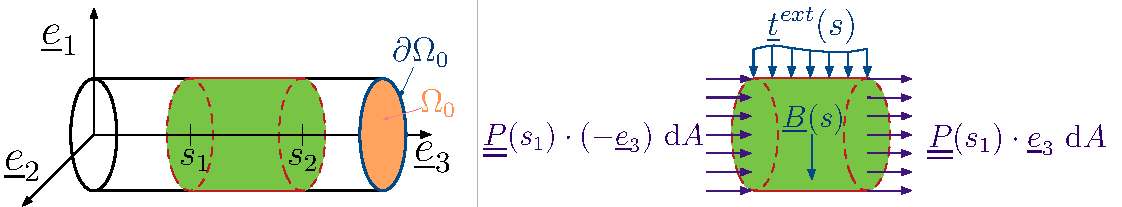
\includegraphics[width=22cm, keepaspectratio=true]{sections/cosserat_rods/images/Forces}
  \end{figure}

  \textbf{external forces}: body force $\underline{B}$ and external traction $\underline{t}^{ext}$
  
  \begin{displaymath}
    \begin{alignedat}{1}
      &\iiint_{\text{undeformed volume}} \underline{B} \dif V + \iint_{\text{lateral surface}} \underline{t}^{ext} \dif A = \\
      = &\int_{s_1}^{s_2} \Biggl( \iint_{\Omega_{0}(s)} \underline{B}(X_1,X_2,s) \dif A + \oint_{\partial \Omega_{0}(s)} \underline{t}^{ext}(l,s) \dif l \Biggr) \dif s =: \\
      =: & \int_{s_1}^{s_2} \underline{\hat{n}}(s) \dif s
    \end{alignedat}
  \end{displaymath}
  % TODO (X_1,X_2,s) bzw. (l,s)
  \vspace{0.5em}
  $\rightarrow$ distributed external load $\underline{\hat{n}}(s)$ (force per unit of undeformed length)
\end{frame}


%-------------------------------------------------------------------------------
\begin{frame}
  \frametitle{Balance of forces (part 2)}

  %\vspace{-0.5em}
  \begin{figure}
    \centering
    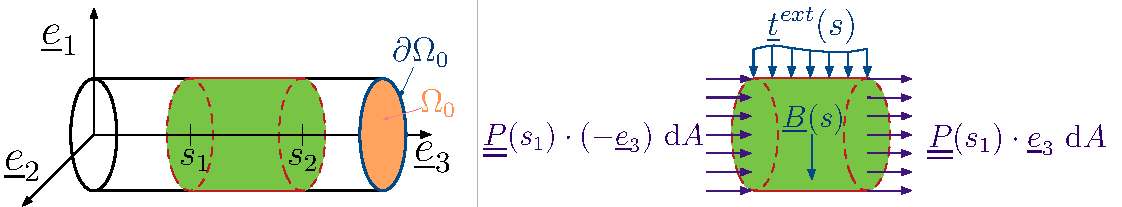
\includegraphics[width=22cm, keepaspectratio=true]{sections/cosserat_rods/images/Forces}
  \end{figure}

  %Material description: $\nabla_{\underline{X}} \cdot \doubleunderline{P} + \underline{B} = \rho_0 \cdot \underline{A}$

  \textbf{internal forces}
  
  \begin{displaymath}
    \begin{alignedat}{1}
      &\iint_{\Omega_0(s)} \doubleunderline{P} \cdot \underline{n} \dif A = \\
      = &\iint_{\Omega_0(s)} \doubleunderline{P}(X_1, X_2, s) \cdot \underline{e}_3 \dif X_1 \dif X_2 = \\
      =: \, &\underline{n}(s)
    \end{alignedat}
  \end{displaymath}
  
  \vspace{0.5em}
  $\rightarrow$ internal contact force $\underline{n}(s)$ (force per unit of undeformed length)
\end{frame}



%-------------------------------------------------------------------------------
\begin{frame}
  \frametitle{Balance of forces (part 3)}
  
  \begin{figure}
    \centering
    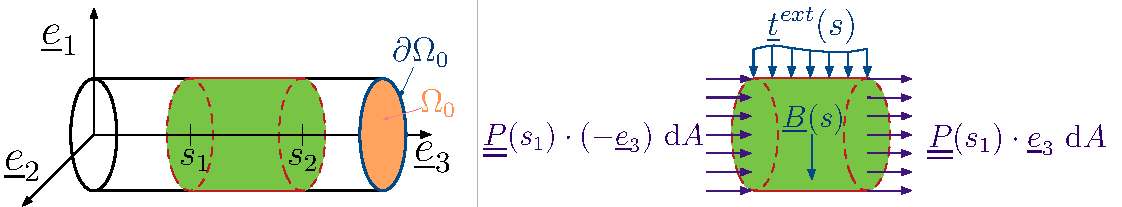
\includegraphics[width=22cm, keepaspectratio=true]{sections/cosserat_rods/images/Forces}
  \end{figure}
  
  \textbf{balance of forces} (statics)
  
  \begin{displaymath}
    \int_{s_1}^{s_2} \underline{\hat{n}}(s) \dif s + \underline{n}(s_2) - \underline{n}(s_1) =
    \int_{s_1}^{s_2} \underline{\hat{n}}(s) + \underline{n}^{\prime}(s) \dif s =
    \underline{0}
  \end{displaymath}
  
  since $s_1$ and $s_2$ are arbitrary cross sections we let $s_2 \to s_1$ \newline
  and obtain the \textbf{local force balance}
  \begin{displaymath}
    \underline{n}^{\prime}(s) + \underline{\hat{n}}(s) = \underline{0}
  \end{displaymath}
  \vspace{0.6em}
  
  \textbf{local balance of linear momentum} (dynamics)
  \begin{displaymath}
    \underline{n}^{\prime}(s) + \underline{\hat{n}}(s) = \rho_0 \, A \, \underline{\ddot{r}}(s)
  \end{displaymath}
\end{frame}


%-------------------------------------------------------------------------------
\begin{frame}
  \frametitle{Balance of moments (part 1)}
  
  we write the moment balance about the origin: $\underline{M} = \underline{x} \times \underline{F}$ \newline
  with $\underline{x}(X_1,X_2,s) = \underline{r}(s) + \bigl( \underline{x}(X_1,X_2,s) - \underline{r}(s) \bigr)$
  \vspace{0.5em}
  
  \textbf{moment due to external loads}
  \begin{displaymath}
    \begin{alignedat}{2}
      &\iiint_{\text{undeformed volume}} \underline{x} \times \underline{B} \dif V + &\\
       + &\iint_{\text{lateral surface}} \underline{x} \times \underline{t}^{ext} \dif A = &\\
      = &\int_{s_1}^{s_2} \Biggl( \underline{r}(s) \times \iint_{\Omega_{0}(s)} \underline{B}(s) \dif A \Biggr) \dif s +
        &\int_{s_1}^{s_2} \Biggl( \iint_{\Omega_{0}(s)} \bigl( \underline{x}(.,.,s) - \underline{r}(s) \bigr) \times \underline{B} \dif A \Biggr) \dif s + \\
        + &\int_{s_1}^{s_2} \Biggl( \underline{r}(s) \times \oint_{\partial \Omega_{0}(s)} \underline{t}^{ext}(s) \dif l \Biggr) \dif s +
        &\int_{s_1}^{s_2} \Biggl( \oint_{\partial \Omega_{0}(s)} \bigl( \underline{x}(.,.,s) - \underline{r}(s) \bigr) \times \underline{t}^{ext} \dif l \Biggr) \dif s =
    \end{alignedat}
  \end{displaymath}
\end{frame}



%-------------------------------------------------------------------------------
\begin{frame}
  \frametitle{Balance of moments (part 2)}
  % TODO use color to show which terms are equal
  \begin{displaymath}
    \begin{alignedat}{1}
      = &\int_{s_1}^{s_2} \Biggl( \underline{r}(s) \times \biggl( \iint_{\Omega_0} \underline{B}(s) \dif A + \oint_{\partial \Omega_{0}(s)} \underline{t}^{ext}(s) \dif l \biggr) \Biggr) \dif s + \\
        + &\int_{s_1}^{s_2} \biggl( \iint_{\Omega_{0}(s)} \bigl( \underline{x}(.,.,s) - \underline{r}(s) \bigr) \times \underline{B}(s) \dif A + \oint_{\partial \Omega_0} \bigl( \underline{x}(.,.,s) - \underline{r}(s) \bigr) \times \underline{t}^{ext}(s) \dif l \biggr) \dif s = \\
      =: &\int_{s_1}^{s_2} \underline{r}(s) \times \underline{\hat{n}}(s) \dif s +
        \int_{s_1}^{s_2} \underline{\hat{m}}(s) \dif s
    \end{alignedat}
  \end{displaymath}
\end{frame}


%-------------------------------------------------------------------------------
\begin{frame}
  \frametitle{Balance of moments (part 3)}
    % TODO use color to show which terms are equal
  \textbf{moment due to internal forces} % TODO tractions (also before with forces)
  \begin{displaymath}
    \begin{alignedat}{1}
      &\iint_{\Omega_0(s)} \underline{x}(X_1,X_2,s) \times \bigl( \doubleunderline{P}(X_1,X_2,s) \cdot \underline{e}_3 \bigr) \dif A = \\
      =&\iint_{\Omega_0(s)} \underline{r}(s) \times \bigl( \doubleunderline{P}(X_1,X_2,s) \cdot \underline{e}_3 \bigr) \dif X_1 \dif X_2 + \\
      + &\iint_{\Omega_0(s)} \bigl( \underline{x}(X_1,X_2,s) - \underline{r}(s) \bigr) \times \bigl( \doubleunderline{P}(X_1,X_2,s) \cdot \underline{e}_3 \bigr) \dif X_1 \dif X_2 = \\
      = \, &\underline{r}(s) \times \iint_{\Omega_0(s)} \doubleunderline{P}(X_1,X_2,s) \cdot \underline{e}_3 \dif X_1 \dif X_2 + \dots = \\
      =: \, &\underline{r}(s) \times \underline{n}(s) + \underline{m}(s)
    \end{alignedat}
  \end{displaymath}
\end{frame}


%-------------------------------------------------------------------------------
\begin{frame}
  \frametitle{Balance of moments (part 4)}
  
  \textbf{balance of moments} (statics)
  \begin{displaymath}
    \begin{alignedat}{1}
      &\int_{s_1}^{s_2} \bigl( \underline{r}(s) \times \underline{\hat{n}}(s) + \underline{\hat{m}}(s)\bigr) \dif s + \\ 
      &+ \bigl( \underline{r}(s_2) \times \underline{n}(s_2) + \underline{m}(s_2) \bigr)
         - \bigl( \underline{r}(s_1) \times \underline{n}(s_1) + \underline{m}(s_1) \bigr) = \\
      &= \int_{s_1}^{s_2} \Bigl( \bigl( \cancel{\underline{r}(s) \times \underline{\hat{n}}(s)} + \underline{\hat{m}}(s) \bigr) + \bigl( \underline{r}^{\prime}(s) \times \underline{n}(s) + \cancel{\underline{r}(s) \times \underline{n}^{\prime}(s)} + \underline{m}^{\prime}(s) \bigr) \Bigr) \dif s = \\
      &= \int_{s_1}^{s_2} \bigl( \underline{\hat{m}}(s) + \underline{r}^{\prime}(s) \times \underline{n}(s) + \underline{m}^{\prime}(s) \bigr) \dif s
    \end{alignedat}
  \end{displaymath}
  % Note: terms canceled because of force balance
  
  since $s_1$ and $s_2$ are arbitrary cross sections we let $s_2 \to s_1$ \newline
  and obtain the \textbf{local moment balance}
  \begin{displaymath}
    \underline{m}^{\prime}(s) + \underline{r}^{\prime}(s) \times \underline{n}(s) + \underline{\hat{m}}(s) = \underline{0}
  \end{displaymath}

  \vspace{0.7em}
  \textbf{local balance of angular momentum} (dynamics)
  \begin{displaymath}
    \underline{m}^{\prime}(s) +
    \underline{r}^{\prime}(s) \times \underline{n}(s) +
    \underline{\hat{m}}(s) =
    \rho_0 \cdot
    \pd{}{t} \bigl( \doubleunderline{I} \cdot \underline{\omega} \bigr)
  \end{displaymath}
\end{frame}


%-------------------------------------------------------------------------------

\begin{frame}
  \frametitle{Review of balance equations (statics)}
  
  \textbf{force balance} (3 equations)
  \begin{displaymath}
    \underline{n}^{\prime}(s) + \underline{\hat{n}}(s) = \underline{0}
  \end{displaymath}
  
  \textbf{moment balance} (3 equations)
  \begin{displaymath}
    \underline{m}^{\prime}(s) + \underline{r}^{\prime}(s) \times \underline{n}(s) + \underline{\hat{m}}(s) = \underline{0}
  \end{displaymath}
  
  \vspace{1em}
  we have \textbf{6 kinematic unknowns}, $\underline{r}(s)$ and $\doubleunderline{R}(s)$ with 3 unknowns each,
  
  \vspace{0.3em}
  and we have \textbf{6 kinetic unknowns}
  \begin{displaymath}
    \begin{alignedat}{1}
      &\underline{n}(s) = \iint_{\Omega_0(s)} \doubleunderline{P}(X_1, X_2, s) \cdot \underline{e}_3 \dif X_1 \dif X_2 \\
      &\underline{m}(s) = \iint_{\Omega_0(s)} \bigl( \underline{x}(X_1,X_2,s) - \underline{r}(s) \bigr) \times \bigl( \doubleunderline{P}(X_1,X_2,s) \cdot \underline{e}_3 \bigr) \dif X_1 \dif X_2
    \end{alignedat}
  \end{displaymath}
  
  \vspace{0.3em}
  to close the system, we need a relationship between the kinematic and the kinetic quantities
  
  \vspace{0.2em}
  $\rightarrow$ this relationship is called \textit{constitutive law of the material}
\end{frame}


%===============================================================================
\subsection{Constitutive laws}

%-------------------------------------------------------------------------------
\begin{frame}
  \frametitle{Motivation of constitutive law}

  let's recall the \textbf{constrained deformation map} (without warping)
  \begin{displaymath}
    \underline{x}(X_1,X_2,s) = \underline{f}(X_1,X_2,s) = \underline{r}(s) + X_{\alpha} \, \underline{d}_{\alpha} = \underline{r}(s) + \doubleunderline{R}(s) \cdot ( X_{\alpha} \, \underline{e}_{\alpha} )
  \end{displaymath}
  
  we compute the \textbf{deformation gradient} and obtain
  % TODO computation of F in more detail?
  \begin{displaymath}
    \begin{alignedat}{1}
      \doubleunderline{F}(X_1,X_2,s) &= \underline{r}^{\prime}(s) \otimes \underline{e}_3 + \doubleunderline{R}(s) \: \underline{e}_{\alpha} \otimes \underline{e}_{\alpha} + \doubleunderline{R}^{\prime}(s) \: X_{\alpha} \underline{e}_{\alpha} \otimes \underline{e}_3 = \\
      &= \doubleunderline{R}(s) \biggl( \doubleunderline{R}^{\mathrm{T}}(s) \, \underline{r}^{\prime}(s) \otimes \underline{e}_3 + \underline{e}_{\alpha} \otimes \underline{e}_{\alpha} + \doubleunderline{R}^{\mathrm{T}}(s) \, \doubleunderline{R}^{\prime}(s) \, X_{\alpha} \underline{e}_{\alpha} \otimes \underline{e}_3 \biggr)
    \end{alignedat}
  \end{displaymath}
  
  \vspace{1em}
  we then obtain an expression of the form
  \begin{displaymath}
    \doubleunderline{P}(X_1,X_2,s) = \mathop{\mathrm{function}}\bigl( \doubleunderline{F}(X_1,X_2,s) \bigr) \, ,
  \end{displaymath}
  
  \vspace{0.4em}
  %which leads us to the constitutive law ...
  from the 3-dimensional constitutive law of the material
\end{frame}



%-------------------------------------------------------------------------------
\begin{frame}
  \frametitle{Example with constrained deformation map: stretching of a bar}
  
  \vspace{-1em}
  \begin{multicols}{2}
    \noindent
    \begin{figure}
      \centering
      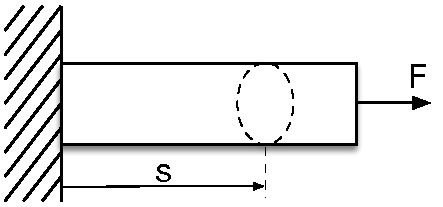
\includegraphics[width=8cm, keepaspectratio=true]{sections/cosserat_rods/images/ExampleConstrainedMapStretchingBar}
    \end{figure}
    
    we have the \textbf{deformed configuration}
    \begin{displaymath}
      \begin{alignedat}{1}
        \underline{r}(s) &= \lambda \, s \, \underline{e}_3 \quad \text{with } \lambda \in \mathbb{R}^{+} \\
        \doubleunderline{R}(s) &= \doubleunderline{I} \\
      \end{alignedat}
    \end{displaymath}
  \end{multicols}
  
  \vspace{-0.5em}
  therefore the \textbf{deformation map} is
  \begin{displaymath}
    \underline{x}(X_1,X_2,s) \underline{x}(s) = \lambda \, s \, \underline{e}_3 + \doubleunderline{I} \cdot (X_{\alpha} \, \underline{e}_{\alpha})
  \end{displaymath}
  
  and its \textbf{deformation gradient} is given by
  \begin{displaymath}
    \doubleunderline{F}(X_1,X_2,s) = \doubleunderline{F}(s) = \lambda \, \underline{e_3} \otimes \underline{e_3} + \underline{e}_{\alpha} \otimes \underline{e}_{\alpha} = (\lambda - 1) \underline{e}_3 \otimes \underline{e}_3 + \doubleunderline{I}  
  \end{displaymath}
  
  but the \textbf{axial force}
  \begin{displaymath}
    \begin{alignedat}{1}
      \underline{n}(s) &= \iint_{\Omega_0(s)} \doubleunderline{P}(X_1, X_2, s) \cdot \underline{e}_3 \dif X_1 \dif X_2 \\
      &\neq E \, A \, (\lambda - 1)
    \end{alignedat}
  \end{displaymath}
  because the deformation map violates the traction-free boundary condition \newline
  $\rightarrow$ the cross section must be able to shrink when the bar is stretched!
\end{frame}


%-------------------------------------------------------------------------------
\begin{frame}
  \frametitle{Constitutive equation for a hyperelastic rod}
  
  note: hyperelasticity refers to a reversible deformation process; \newline
  therefore it can be described by a potential function
  
  \vspace{0.7em}
  in order to derive constitutive laws from theory, \newline
  we will use functions that are potentials of internal energy ... 
  
  \vspace{1.5em}
  \textbf{strain energy per unit of undeformed length}
  \begin{displaymath}
    \phi = \phi \bigl( \underline{r}(s),\doubleunderline{R}(s),\underline{r}^{\prime}(s),\doubleunderline{R}^{\prime}(s) \bigr)
  \end{displaymath}
  
  \vspace{1.5em}
  \textbf{strain energy per unit of undeformed volume}
  \begin{displaymath}
    W \bigl( \cancel{\underline{f}(s)}, \doubleunderline{F}(s), \cancel{\nabla \doubleunderline{F}(s)} \bigr) = W \bigl( \doubleunderline{F}(s) \bigr)
  \end{displaymath}

  \vspace{0.1em}
  \begin{itemize}
    \item $\underline{f}(s)$ canceled because of principle of frame-indifference
    \item $\nabla \doubleunderline{F}(s)$ canceled because we will not consider higher order derivatives of the deformation map in classical elasticity (compared to higher gradient elasticity theory)
    % discontinuities at interfaces in the material 
  \end{itemize}
\end{frame}


%-------------------------------------------------------------------------------
\begin{frame}
  \frametitle{Principle of material frame-indifference (part 1)}

  \vspace{-0.5em}
  \begin{itemize}
    \item  constitutive laws should be invariant with regard to the external frame of reference, \newline i.e. the coordinate system ($\rightarrow$ observer objectivity)
    \item $\Rightarrow$ rigid body motions do not affect the internally stored energy in the system, \newline \null \quad (i.e. the mechanical/deformation energy)
    \item $\rightarrow$ we want to identify a set of strain measures which is invariant to rigid body motions!
  \end{itemize}
  
  \vspace{0.3em}
  to that end we set up a simple \textbf{thought experiment}
  \begin{itemize}
    \item perform two rigid body motions: one rotation followed by one translation
    \item equate the internal mechanical energy potentials: $\eval[1]{\phi}_{\alpha} = \eval[1]{\phi}_{\beta} = \eval[1]{\phi}_{\gamma}$
  \end{itemize}
  
  \vspace{-1.4em}
  \begin{figure}
    \centering
    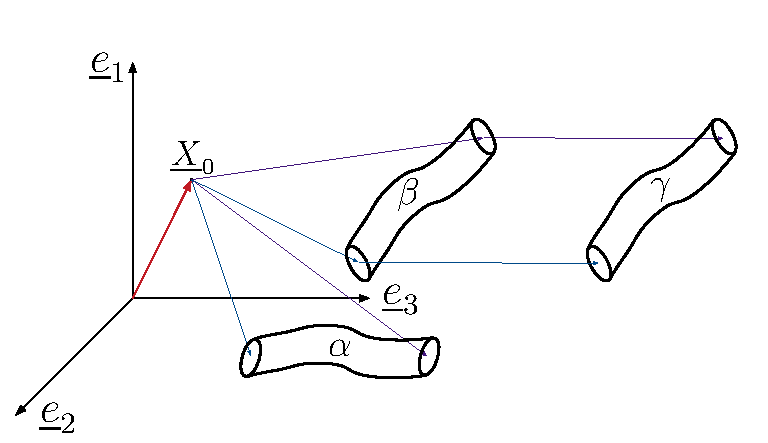
\includegraphics[width=13cm, keepaspectratio=true]{sections/cosserat_rods/images/FrameIndifferenceExperiment}
  \end{figure}  
\end{frame}


%-------------------------------------------------------------------------------
\begin{frame}
  \frametitle{Principle of material frame-indifference (part 2)}
  % TODO split slide
  \vspace{-0.6em}
  \begin{enumerate}
    \item initial configuration $\alpha$
      \begin{itemize}
        \item centerline given by $\underline{r}^{\alpha}(s)$
        \item cross section orientation given by $\doubleunderline{R}^{\alpha}(s)$
        \item energy potential given by $\eval[1]{\phi}_{\beta}(s) = \phi \bigl( \underline{r}^{\alpha}{\alpha}(s) , \, \doubleunderline{R}^{\alpha}(s) , \, \underline{r}^{\alpha \prime}(s) , \, \doubleunderline{R}^{\alpha \prime}(s) \bigr)$
      \end{itemize}
      
    \item configuration $\beta$ after rigid body rotation by some $\doubleunderline{Q} \in SO(3)$ about some $\underline{X}_0 \in \mathbb{R}^3$
      \begin{itemize}
        \item $\underline{r}^{\beta}(s) = \underline{X}_0 + \doubleunderline{Q} \left( \underline{r}^{\alpha}(s) - \underline{X}_0 \right) \quad \Rightarrow \quad \underline{r}^{\beta \prime}(s) = \doubleunderline{Q} \, \underline{r}^{\alpha \prime}(s)$ \newline
          \null \quad (shift coordinate system s.t. rotation's fix-point $\hat{=}$ origin; rotate; undo shift)
        \item $\doubleunderline{R}^{\beta}(s) = \doubleunderline{Q} \, \doubleunderline{R}^{\alpha}(s) \quad \Rightarrow \quad \doubleunderline{R}^{\beta \prime}(s) = \doubleunderline{Q} \, \doubleunderline{R}^{\alpha \prime}(s)$
        \item $\eval[1]{\phi}_{\beta}(s) = \phi \bigl( \underline{X}_0 + \doubleunderline{Q} \left( \underline{r}^{\alpha}(s) - \underline{X}_0 \right) , \, \doubleunderline{Q} \, \doubleunderline{R}^{\alpha}(s) , \, \doubleunderline{Q} \, \underline{r}^{\alpha \prime}(s) , \, \doubleunderline{Q} \, \doubleunderline{R}^{\alpha \prime}(s) \bigr)$
      \end{itemize}
      
    \item configuration $\gamma$ after rigid body translation by some $\underline{t} \in \mathbb{R}^3$
      \begin{itemize}
        \item $\underline{r}^{\gamma}(s) = \underline{X}_0 + \doubleunderline{Q} \left( \underline{r}^{\alpha}(s) - \underline{X}_0 \right) + \underline{t} \quad \Rightarrow \quad \underline{r}^{\gamma \prime}(s) = \underline{r}^{\beta \prime}(s) = \doubleunderline{Q} \,\underline{r}^{\alpha \prime}(s)$
        \item $\doubleunderline{R}^{\gamma}(s) = \doubleunderline{I} \, \doubleunderline{R}^{\beta}(s) = \doubleunderline{Q} \, \doubleunderline{R}^{\alpha}(s) \quad \Rightarrow \quad \doubleunderline{R}^{\gamma \prime}(s) = \doubleunderline{R}^{\beta \prime}(s) = \doubleunderline{Q} \, \doubleunderline{R}^{\alpha \prime}(s)$
        \item $\eval[1]{\phi}_{\gamma}(s) = \phi \bigl( \underline{X}_0 + \doubleunderline{Q} \left( \underline{r}^{\alpha}(s) - \underline{X}_0 \right) + \underline{t} , \, \doubleunderline{Q} \, \doubleunderline{R}^{\alpha}(s) , \, \doubleunderline{Q} \,\underline{r}^{\alpha \prime}(s) , \, \doubleunderline{Q} \, \doubleunderline{R}^{\alpha \prime}(s) \bigr)$
      \end{itemize}
  \end{enumerate}
\end{frame}



%-------------------------------------------------------------------------------
\begin{frame}
  \frametitle{Principle of material frame-indifference (part 3)}
  
  comparing $\eval[1]{\phi}_{\beta}(s) \overset{!}{=} \eval[1]{\phi}_{\gamma}(s)$ gives
  \begin{displaymath}
    \begin{alignedat}{4}
      \phi \bigl(
        &\underline{X}_0 + \doubleunderline{Q} \left( \underline{r}^{\alpha}(s) - \underline{X}_0 \right) , \,
        &\doubleunderline{Q} \, \doubleunderline{R}^{\alpha}(s) , \,
        &\doubleunderline{Q} \, \underline{r}^{\alpha \prime}(s) , \,
        &\doubleunderline{Q} \, \doubleunderline{R}^{\alpha \prime}(s)
      \bigr) = \\
      \phi \bigl(
        &\underline{X}_0 + \doubleunderline{Q} \left( \underline{r}^{\alpha}(s) - \underline{X}_0 \right) + \underline{t} , \,
        &\doubleunderline{Q} \, \doubleunderline{R}^{\alpha}(s) , \,
        &\doubleunderline{Q} \, \underline{r}^{\alpha \prime}(s) , \,
        &\doubleunderline{Q} \, \doubleunderline{R}^{\alpha \prime}(s)
      \bigr) \Rightarrow
    \end{alignedat}
  \end{displaymath}
  $\Rightarrow \phi$ is independent of $\underline{r}(s)$, i.e. the first argument can be omitted
  
  \vspace{1em}
  without loss of generality we can set the arbitrarily chosen rotation matrix $\doubleunderline{Q} := \doubleunderline{R}^{\mathrm{T}}$
  \begin{displaymath}
    \phi(s) = \phi \bigl(
        . , \,
        \doubleunderline{R}^{\mathrm{T}}(s) \, \doubleunderline{R}(s) , \,
        \doubleunderline{R}^{\mathrm{T}}(s) \, \underline{r}^{\prime}(s) , \,
        \doubleunderline{R}^{\mathrm{T}}(s) \, \doubleunderline{R}^{\prime}(s)
      \bigr)
  \end{displaymath}
  
  \vspace{1em}
  we define a new version of $\phi$ that depends only on the invariants
  \begin{displaymath}
    \psi(s) := \psi \bigl(
      \doubleunderline{R}^{\mathrm{T}}(s) \, \underline{r}^{\prime}(s) , \,
      \doubleunderline{R}^{\mathrm{T}}(s) \, \doubleunderline{R}^{\prime}(s)
    \bigr)
  \end{displaymath}  
\end{frame}


%-------------------------------------------------------------------------------
\begin{frame}
  \frametitle{Invariant strain measures (part 1)}
  
  
  we can verify that $\doubleunderline{R}^{\mathrm{T}} \, \underline{r}^{\prime}$ and $\doubleunderline{R}^{\mathrm{T}} \, \doubleunderline{R}^{\prime}$ are truly invariant strain measures:
  
  \vspace{1em}
  we get
  \begin{displaymath}
    \doubleunderline{R}^{\gamma \mathrm{T}} \, \underline{r}^{\gamma \prime} =
    \bigl( \doubleunderline{Q} \, \doubleunderline{R}^{\alpha} \bigr)^{\mathrm{T}} \, \bigl( \doubleunderline{Q} \, \underline{r}^{\alpha \prime} \bigr) =
    \bigl( \doubleunderline{R}^{\alpha \mathrm{T}} \, \doubleunderline{Q}^{\mathrm{T}} \bigr) \, \bigl( \doubleunderline{Q} \, \underline{r}^{\alpha \prime} \bigr) =
    \doubleunderline{R}^{\alpha \mathrm{T}} \, \underline{r}^{\alpha \prime}
  \end{displaymath}
  and
  \begin{displaymath}
    \doubleunderline{R}^{\gamma \mathrm{T}} \, \doubleunderline{R}^{\gamma \prime} =
    \bigl( \doubleunderline{Q} \, \doubleunderline{R}^{\alpha} \bigr)^{\mathrm{T}} \, \bigl( \doubleunderline{Q} \, \doubleunderline{R}^{\alpha \prime} \bigr) =
    \bigl( \doubleunderline{R}^{\alpha \mathrm{T}} \, \doubleunderline{Q}^{\mathrm{T}} \bigr) \, \bigl( \doubleunderline{Q} \, \doubleunderline{R}^{\alpha \prime} \bigr) =
    \doubleunderline{R}^{\alpha \mathrm{T}} \, \doubleunderline{R}^{\alpha \prime}
  \end{displaymath}
\end{frame}


%-------------------------------------------------------------------------------
\begin{frame}
  \frametitle{Invariant strain measures (part 2)}
  we define $\underline{v}$ as the shorthand for the first invariant
  \begin{displaymath}
    \underline{v} =
    \begin{bmatrix} v_1 \\ v_2 \\ v_3 \end{bmatrix} = 
    v_i \, \underline{e}_i :=
    \doubleunderline{R}^{\mathrm{T}} \, \underline{r}^{\prime}
    \quad \Rightarrow \quad
    \underline{r}^{\prime} =
    \doubleunderline{R} \, \underline{v} =
    v_i \, \doubleunderline{R} \, \underline{e}_i =
    v_i \, \underline{d}_i
  \end{displaymath}
  
  and from orthogonality of the director basis ($\underline{d}_i \cdot \underline{d}_j = \delta_{ij}$) it follows that $v_i = \underline{r}^{\prime} \cdot \underline{d}_i$
  
  \vspace{0.3em}
  $\rightarrow \underline{v} = \doubleunderline{R}^{\mathrm{T}} \, \underline{r}^{\prime}$ is the centerline tangent vector resolved in the local director basis!
  
  \vspace{1em}
  more specifically we have ...
  \begin{itemize}
    \item $v_1 = \underline{r}^{\prime} \, \underline{d}_1$ : rate of transverse shift $\hat{=}$ shear along $\underline{d}_1$
    \item $v_2 = \underline{r}^{\prime} \, \underline{d}_2$ : shear along $\underline{d}_2$
    \item $v_3 = \underline{r}^{\prime} \, \underline{d}_3$ : rate of axial shift $\hat{=}$ axial stretch 
  \end{itemize}
  % TODO make a figure
\end{frame}


%-------------------------------------------------------------------------------
\begin{frame}
  \frametitle{Invariant strain measures (part 3)}
  
  we define $\doubleunderline{K}$ as the shorthand for the second invariant
  \begin{displaymath}
    \doubleunderline{K} =
    K_{ij} \, \underline{e}_i \otimes \underline{e}_j :=
    \doubleunderline{R}^{\mathrm{T}} \, \doubleunderline{R}^{\prime}
  \end{displaymath}
  
  \vspace{0.5em}
  \textbf{proof} that $\doubleunderline{K}$ is \textit{skew-symmetric} ($K_{ij} = -K_{ji}$)
  \begin{displaymath}
    \doubleunderline{R}^{\mathrm{T}} \, \doubleunderline{R} = \doubleunderline{I}
    \quad \Rightarrow \quad
    \doubleunderline{R}^{\mathrm{T}} \, \doubleunderline{R}^{\prime} + \doubleunderline{R}^{\prime \mathrm{T}} \, \doubleunderline{R} = \doubleunderline{0}
    \quad \Rightarrow \quad
    \doubleunderline{K} = -\doubleunderline{K}^{\mathrm{T}}
  \end{displaymath}
  
  \vspace{0.5em}
  we therefore can write
  \begin{displaymath}
    \doubleunderline{K} = 
    \begin{bmatrix}
       0   & -k_3 &  k_2 \\
       k_3 &  0   & -k_1 \\
      -k_2 &  k_1 &  0
    \end{bmatrix}
  \end{displaymath}
  \vspace{0.5em}
  and we recall that $\doubleunderline{K} \, \underline{a} = \underline{k} \times \underline{a} \: \forall \underline{a} \in \mathbb{R}^3$ with $\underline{k} = \axial(\doubleunderline{K}) = k_i \, \underline{e}_i$
  
  \vspace{1em}
  $\rightarrow$ with $\left( \underline{v} , \, \underline{k} \right)$ we have the 6 strain measures given in the frame of the director basis! \newline
  $\rightarrow$ $\psi = \psi \bigl( \underline{v} , \, \doubleunderline{K} \bigr) =: \hat{\psi} \bigl( \underline{v} , \, \underline{k} \bigr)$ (for easy notation we will drop the $\hat{.}$ in the sequel)
\end{frame}


%-------------------------------------------------------------------------------
\begin{frame}
  \frametitle{Invariant strain measures (part 4)}

  to better understand the physical meaning of $\underline{k}$ we have a look at two examples ...
  
  \vspace{0.5em}
  \textbf{pure twisting of a rod}
  \vspace{-1em}
  \begin{multicols}{2}
    \noindent
    
    \begin{figure}
      \centering
      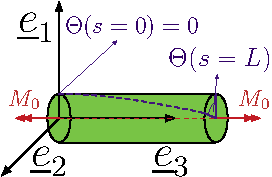
\includegraphics[width=10cm, keepaspectratio=true]{sections/cosserat_rods/images/PureTwistingExample}
    \end{figure}

    \begin{itemize}
      \item rotation of cross sections around $\underline{e}_3$-axis
      \item angle of rotation for the cross section at $s$ given by $\Theta(s) = \Theta^{\prime} \cdot s$ \newline
        with $\Theta^{\prime} = const.$ because external moments act only at $s=0$ and $s=L$
    \end{itemize}
    \vspace{0.1em}
    \begin{displaymath}
      \underline{r}(s) = s \cdot \underline{e}_3 
      \: \Rightarrow \:
      \underline{r}^{\prime}(s) = \underline{e}_3
    \end{displaymath}
    \begin{displaymath}
      \: \Rightarrow \:
      \underline{v} = \doubleunderline{R}^{\mathrm{T}} \, \underline{r}^{\prime} =
      \begin{bmatrix}
        0 & 0 & 1
      \end{bmatrix}^{\mathrm{T}}
      \: \Rightarrow \:
      v_3 = 1
    \end{displaymath}
%    \begin{displaymath}
%      \underline{r}(s) = s \cdot \underline{e}_3 
%      \: \Rightarrow \:
%      \underline{r}^{\prime}(s) = \underline{e}_3
%      \: \Rightarrow \:
%      \underline{v} = \doubleunderline{R}^{\mathrm{T}} \, \underline{r}^{\prime} =
%      \begin{bmatrix}
%        0 & 0 & 1
%      \end{bmatrix}^{\mathrm{T}}
%      \: \Rightarrow \:
%      v_3 = 1
%    \end{displaymath}
  \end{multicols}
  \vspace{-1.2em}
  \begin{displaymath}
    \doubleunderline{R}(s) =
    \begin{bmatrix}
      +\cos(\Theta(s)) & -\sin(\Theta(s)) & 0 \\
      +\sin(\Theta(s)) & +\cos(\Theta(s)) & 0 \\
      0 & 0 & 1
    \end{bmatrix}
    \: \Rightarrow \:
    \doubleunderline{R}^{\prime}(s) =
    \Theta^{\prime} \cdot
    \begin{bmatrix}
      -\sin(\Theta(s)) & -\cos(\Theta(s)) & 0 \\
      +\cos(\Theta(s)) & -\sin(\Theta(s)) & 0 \\
      0 & 0 & 0
    \end{bmatrix}
  \end{displaymath}
    
  \begin{displaymath}
    \doubleunderline{K}(s) =
    \doubleunderline{R}^{\mathrm{T}}(s) \, \doubleunderline{R}^{\prime}(s) =
    \begin{bmatrix}
      0 & -\Theta^{\prime} & 0 \\
      +\Theta^{\prime} & 0 & 0 \\
      0 & 0 & 0
    \end{bmatrix}
    \: \Rightarrow \:
    \underline{k} =
    \begin{bmatrix}
      0 \\ 0 \\ \Theta^{\prime}
    \end{bmatrix}
    \: \Rightarrow \:
    k_3 = \Theta^{\prime}
  \end{displaymath}
\end{frame}

%-------------------------------------------------------------------------------
\begin{frame}
  \frametitle{Invariant strain measures (part 5)}

  \textbf{pure bending of a rod}
  \begin{multicols}{2}
    \noindent
    \begin{figure}
      \centering
      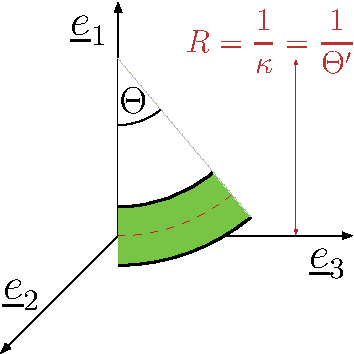
\includegraphics[width=8cm, keepaspectratio=true]{sections/cosserat_rods/images/PureBendingExample}
    \end{figure}
    
    \begin{itemize}
      \item rotation of cross sections around $\underline{e}_2$-axis
      \item angle of rotation for the cross section at $s$ given by $\Theta(s) = \Theta^{\prime} \cdot s = \kappa \cdot s$\newline
        with $\Theta^{\prime} = \kappa = const.$ because external moments act only at $s=0$ and $s=L$
    \end{itemize}
    \vspace{0.1em}
    \begin{displaymath}
      \underline{r}(s) = s \cdot \underline{e}_3 
      \: \Rightarrow \:
      \underline{r}^{\prime}(s) = \underline{e}_3
    \end{displaymath}
    \begin{displaymath}
      \: \Rightarrow \:
      \underline{v} = \doubleunderline{R}^{\mathrm{T}} \, \underline{r}^{\prime} =
      \begin{bmatrix}
        0 & 0 & 1
      \end{bmatrix}^{\mathrm{T}}
      \: \Rightarrow \:
      v_3 = 1
    \end{displaymath}
    \vspace{0.6em}
  \end{multicols}  

  \vspace{-2em}
  \begin{displaymath}
    \doubleunderline{R}(s) =
    \begin{bmatrix}
      +\cos(\Theta(s)) & 0 & +\sin(\Theta(s))\\
      0 & 1 & 0 \\
      -\sin(\Theta(s)) & 0 & +\cos(\Theta(s))
    \end{bmatrix}
    \: \Rightarrow \:
    \doubleunderline{R}^{\prime}(s) =
    \Theta^{\prime} \cdot
    \begin{bmatrix}
      -\sin(\Theta(s)) & 0 & +\cos(\Theta(s))\\
      0 & 0 & 0 \\
      -\cos(\Theta(s)) & 0 & -\sin(\Theta(s))
    \end{bmatrix}
  \end{displaymath}
  
  \begin{displaymath}
    \doubleunderline{K}(s) =
    \doubleunderline{R}^{\mathrm{T}}(s) \, \doubleunderline{R}^{\prime}(s) =
    \begin{bmatrix}
      0 & 0 & +\Theta^{\prime} \\
      0 & 0 & 0 \\
      -\Theta^{\prime} & 0 & 0
    \end{bmatrix}
    \: \Rightarrow \:
    \underline{k} =
    \begin{bmatrix}
      0 \\ \Theta^{\prime} \\ 0
    \end{bmatrix}
    \: \Rightarrow \:
    k_2 = \Theta^{\prime}
  \end{displaymath}
\end{frame}

%-------------------------------------------------------------------------------
\begin{frame}
  % TODO recap slide
  \frametitle{Recap of what we have so far}
  \textbf{balance equations} (in terms of nominal stresses in the reference configuration)
  \begin{displaymath}
    \underline{n}^{\prime} + \underline{\hat{n}} = \underline{0}
    \quad \text{ and } \quad
    \underline{m}^{\prime} + \underline{r}^{\prime} \times \underline{n} + \underline{\hat{m}} = \underline{0}
  \end{displaymath}
  
  \vspace{1.2em}
  \textbf{kinematic quantities $\underline{v}$, $\underline{k}$} \newline
  $\rightarrow$ local strain measures
  \begin{itemize}
    \item $v_1$, $v_2$, $v_3$ : shear along $d_1$, shear along $d_2$, and stretch along $d_3$, respectively
    \item $k_1$, $k_2$, $k_3$ : curvature about $d_1$-, curvature about $d_2$-, and twist about  $d_3$-axis, % \newline \null \quad \quad \quad \quad \quad respectively
  \end{itemize}
  
  \vspace{1.2em}
  \textbf{deformation energy per unit of undeformed length} \newline
  \begin{displaymath}
    \psi \bigl( \doubleunderline{R}^{\mathrm{T}} \, \underline{r}^{\prime} , \, \doubleunderline{R}^{\mathrm{T}} \, \doubleunderline{R}^{\prime} \bigr) =
    \psi \bigl( \underline{v} , \, \doubleunderline{K} \bigr) =
    \psi \bigl( \underline{v} , \, \underline{k} \bigr)
  \end{displaymath}
  
  \vspace{0.5em}
  % TODO Preview?
  $\rightarrow$ derivative of $\psi$ with respect to strains $\underline{v}$, $\underline{k}$ will render stress measures (resolved in the local director basis)
    
    

  
\end{frame}


%-------------------------------------------------------------------------------
\begin{frame}
  \frametitle{Minimum potential energy method (part 1)}
  
  we consider a system consisting of a beam with and an external load $P$ at $s=L$
  
  \vspace{-0.3em}
  \begin{figure}
    \centering
    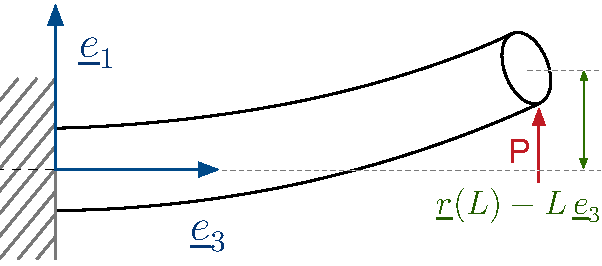
\includegraphics[width=14cm, keepaspectratio=true]{sections/cosserat_rods/images/MinimumPotentialEnergyMethodExample}
  \end{figure}
  
  the \textbf{total energy of the closed system} is given by
  \begin{displaymath}
    \Pi \bigl( \underline{r}, \, \doubleunderline{R} \bigr) =
    \int_0^L \psi \bigl( \underline{v} , \, \underline{k} \bigr) \dif s - P \, \underline{e}_1 \cdot \underline{r}(L)
  \end{displaymath}
  note regarding minus sign: load performs work on the beam, \newline
  thereby lowering the load's potential and also the potential of the closed system
  
  \vspace{0.3em}
  $\rightarrow$ we now want to identify the conditions for a minimum of $\Pi$
\end{frame}


%-------------------------------------------------------------------------------
\begin{frame}
  \frametitle{Minimum potential energy method (part 2)}
  
  \textbf{perturbed versions of $\underline{r}$ and $\doubleunderline{R}$}
  \begin{displaymath}
    \underline{r}_{\epsilon}(s) = \underline{r}(s) + \epsilon \cdot \delta \underline{r}(s)
  \end{displaymath}
  \vspace{-0.5em}
  \begin{displaymath}
    \doubleunderline{R}_{\epsilon}(s) = \underbrace{\xcancel{\doubleunderline{R}(s) + \epsilon \cdot \delta \doubleunderline{R}(s)}}_{\notin SO(3)} = \underbrace{\exp \bigl( \epsilon \cdot \delta \doubleunderline{\Theta}(s) \bigr)}_{\in SO(3)} \, \doubleunderline{R}(s)
    \quad \text{ with } \quad
    \delta \underline{\Theta} := \axial \bigl( \delta \doubleunderline{\Theta} \bigr)
  \end{displaymath}
  
  \vspace{0.6em}
  \textbf{perturbed version of total energy}
  \begin{displaymath}
    \Pi \bigl( \underline{r}_{\epsilon}, \, \doubleunderline{R}_{\epsilon} \bigr) =
    \int_0^L \psi \bigl( \underline{v}_{\epsilon} , \, \underline{k}_{\epsilon} \bigr) \dif s - P \, \underline{e}_1 \cdot \underline{r}_{\epsilon}(L) \overset{!}{=}
    \Pi \bigl( \underline{r}, \, \doubleunderline{R} \bigr) + \epsilon \cdot \delta \Pi \bigl( \underline{r}, \, \doubleunderline{R} \bigr) + \mathcal{o}(\epsilon)
  \end{displaymath}
  
  \vspace{0.6em}
  \textbf{first variation of total energy}
  \begin{displaymath}
    \delta \Pi = \pd{\Pi}{\epsilon} \sVert[3]_{\epsilon=0} =
    \int_0^L \biggl(
    \pd{\psi}{\underline{v}}(s) \cdot \underbrace{ \pd{\underline{v}_{\epsilon}}{\epsilon}(s) \sVert[2]_{\epsilon=0} }_{\delta \underline{v}(s)} +
    \pd{\psi}{\underline{k}}(s) \cdot \underbrace{ \pd{\underline{k}_{\epsilon}}{\epsilon}(s)\sVert[2]_{\epsilon=0} }_{\delta \underline{k}(s)}
    \biggr) \dif s
    - P \, \underline{e}_1 \cdot \pd{\underline{r}_{\epsilon}}{\epsilon}(L) \sVert[3]_{\epsilon=0}
  \end{displaymath}
  
  in the sequel we will work on the terms $\delta \underline{v}(s)$ and $\delta \underline{k}(s)$
\end{frame}


%-------------------------------------------------------------------------------
\begin{frame}
  \frametitle{Minimum potential energy method (part 3)}
  % TODO use of \Delta vs \delta
  % also: \pd{}{\epsilon} vs \od{}{\epsilon}
  \textbf{perturbed version of $\underline{v}$}
  \begin{displaymath}
    \underline{v}_{\epsilon}(s) =
    \doubleunderline{R}_{\epsilon}^{\mathrm{T}}(s) \cdot \underline{r}_{\epsilon}^{\prime}(s) =
    \doubleunderline{R}^{\mathrm{T}}(s) \cdot \biggl( \exp \bigl( \epsilon \cdot \delta \doubleunderline{\Theta}(s) \bigr) \biggr)^{\mathrm{T}} \cdot \bigl( \underline{r}^{\prime}(s) + \epsilon \cdot \delta \underline{r}^{\prime}(s) \bigr)
  \end{displaymath}
  
  \vspace{0.5em}
  \textbf{first variation of $\underline{v}$}
  \begin{displaymath}
    \delta \underline{v}(s) = 
    \pd{\underline{v}_{\epsilon}}{\epsilon}(s) \sVert[3]_{\epsilon=0} =
    \doubleunderline{R}^{\mathrm{T}}(s) \cdot
    \pd{}{\epsilon} \biggl( \exp \bigl( \epsilon \cdot \delta \doubleunderline{\Theta}(s) \bigr) \biggr)^{\mathrm{T}} \sVert[3]_{\epsilon=0}
     \cdot \underline{r}^{\prime}(s) +
     \doubleunderline{R}^{\mathrm{T}}(s) \cdot \delta \underline{r}^{\prime}(s)
  \end{displaymath}
  
  \vspace{0.5em}
  \begin{displaymath}
    \pd{}{\epsilon} \biggl( \exp \bigl( \epsilon \cdot \delta \doubleunderline{\Theta}(s) \bigr) \biggr)^{\mathrm{T}} \sVert[3]_{\epsilon=0} =
    \pd{}{\epsilon} \biggl( \doubleunderline{I} + \epsilon \cdot \delta \doubleunderline{\Theta} + \frac{\epsilon^2}{2} \cdot \delta \doubleunderline{\Theta}^2 + \dots \biggr)^{\mathrm{T}} \sVert[3]_{\epsilon=0} =
    \bigl( \delta \doubleunderline{\Theta} \bigr)^{\mathrm{T}} = -\delta \doubleunderline{\Theta} 
  \end{displaymath}
  
  \vspace{0.5em}
  \begin{displaymath}
    \Rightarrow
    \delta \underline{v}(s) =
    \doubleunderline{R}^{\mathrm{T}}(s) \cdot
    \bigl( - \delta \doubleunderline{\Theta}(s) \cdot \underline{r}^{\prime}(s) + \delta \underline{r}^{\prime}(s) \bigr)
  \end{displaymath}
\end{frame}



%-------------------------------------------------------------------------------
\begin{frame}
  \frametitle{Minimum potential energy method (part 4)}
  
  \textbf{perturbed version of $\doubleunderline{K}$, respectively $\underline{k}$}
  \begin{displaymath}
    \doubleunderline{K}_{\epsilon}(s) =
    \doubleunderline{R}_{\epsilon}^{\mathrm{T}}(s) \cdot \doubleunderline{R}_{\epsilon}^{\prime}(s)
    \quad \text{ and } \quad
    \underline{k}_{\epsilon}(s) = \axial \bigl( \doubleunderline{K}_{\epsilon}(s) \bigr)
  \end{displaymath}
  
  \vspace{0.5em}
  \textbf{first variation of $\underline{k}$}
  \begin{displaymath}
    \delta \underline{k}(s) =
    \pd{\underline{k}_{\epsilon}}{\epsilon}(s) \sVert[3]_{\epsilon=0} =
    \pd{}{\epsilon} \biggl( \axial \bigl( \doubleunderline{R}_{\epsilon}^{\mathrm{T}}(s) \cdot \doubleunderline{R}_{\epsilon}^{\prime}(s) \bigr) \biggr) \sVert[3]_{\epsilon=0} =
  \end{displaymath}
  \begin{displaymath}
    = \axial \biggl( \pd{}{\epsilon} \bigl( \doubleunderline{R}_{\epsilon}^{\mathrm{T}}(s) \cdot \doubleunderline{R}_{\epsilon}^{\prime}(s) \bigr) \sVert[2]_{\epsilon=0} \biggr) \overset{(1)}{=}
    \axial \bigl( \doubleunderline{R}^{\mathrm{T}}(s) \cdot \delta \doubleunderline{\Theta}^{\prime}(s) \cdot \doubleunderline{R} \bigr) \overset{(2)}{=}
    \doubleunderline{R}^{\mathrm{T}}(s) \cdot \delta \underline{\Theta}^{\prime}(s)      
  \end{displaymath}
  
  \vspace{0.5em}
  regarding equality $(2)$ we have ...
  \begin{displaymath}
    \bigl( \doubleunderline{R}^{\mathrm{T}} \cdot \delta \doubleunderline{\Theta}^{\prime} \cdot \doubleunderline{R} \bigr) \cdot \underline{a} =
    \doubleunderline{R}^{\mathrm{T}} \cdot \delta \doubleunderline{\Theta}^{\prime} \cdot \bigl( \doubleunderline{R} \cdot \underline{a} \bigr) =
    \doubleunderline{R}^{\mathrm{T}} \cdot \biggl( \delta \underline{\Theta}^{\prime} \times \bigl( \doubleunderline{R} \cdot \underline{a} \bigr) \biggr) =
    \bigl( \doubleunderline{R}^{\mathrm{T}} \cdot \delta \underline{\Theta}^{\prime} \bigr) \times \underline{a}
  \end{displaymath}
\end{frame}


%-------------------------------------------------------------------------------
\begin{frame}
  \frametitle{Minimum potential energy method (part 5)}
  
  and regarding equality $(1)$ we have ...
  \begin{displaymath}
    \pd{}{\epsilon} \bigl( \doubleunderline{R}_{\epsilon}^{\mathrm{T}}(s) \cdot \doubleunderline{R}_{\epsilon}^{\prime}(s) \bigr) \sVert[2]_{\epsilon=0} =
  \end{displaymath}
  \begin{displaymath}
    = \pd{}{\epsilon} \Biggl[
      \doubleunderline{R}^{\mathrm{T}} \cdot \biggl( \exp \bigl( \epsilon \cdot \delta \doubleunderline{\Theta} \bigr) \biggr)^{\mathrm{T}}
      \cdot \Biggl(
        \biggl( \exp \bigl( \epsilon \cdot \delta \doubleunderline{\Theta} \bigr) \biggr)^{\prime} \cdot \doubleunderline{R}
        + \exp \bigl( \epsilon \cdot \delta \doubleunderline{\Theta} \bigr) \cdot \doubleunderline{R}^{\prime}
      \Biggr)
    \Biggr] \sVert[4]_{\epsilon=0} =
  \end{displaymath}
  \begin{displaymath}
    = \Bigl[
      \cancel{-\doubleunderline{R}^{\mathrm{T}} \cdot \delta \doubleunderline{\Theta} \cdot \doubleunderline{R}^{\prime}} +
        \doubleunderline{R}^{\mathrm{T}} \cdot
        \biggl(
          \delta \doubleunderline{\Theta}^{\prime} \cdot \doubleunderline{R} +
          \cancel{ \delta \doubleunderline{\Theta} \cdot \doubleunderline{R}^{\prime} } 
        \biggr)
      \Bigr] =
      \doubleunderline{R}^{\mathrm{T}} \cdot
      \delta \doubleunderline{\Theta}^{\prime} \cdot \doubleunderline{R}
  \end{displaymath}
  
  \vspace{0.5em}
  ... where we used ...
  \begin{displaymath}
    \pd{}{\epsilon} \biggl( \exp \bigl( \epsilon \cdot \delta \doubleunderline{\Theta}(s) \bigr) \biggr)^{\prime} \sVert[3]_{\epsilon=0} =
    \pd{}{\epsilon} \biggl( \doubleunderline{I} + \epsilon \cdot \delta \doubleunderline{\Theta} + \frac{\epsilon^2}{2} \cdot \delta \doubleunderline{\Theta}^2 + \dots \biggr)^{\prime} \sVert[3]_{\epsilon=0} =
  \end{displaymath}
  \begin{displaymath}
    = \pd{}{\epsilon} \biggl( \epsilon \cdot \delta \doubleunderline{\Theta}^{\prime} + \frac{\epsilon^2}{2} \cdot \delta \doubleunderline{\Theta}^{\prime 2} + \dots \biggr)^{\prime} \sVert[3]_{\epsilon=0} =
    \delta \doubleunderline{\Theta}^{\prime} 
  \end{displaymath}
\end{frame}


%-------------------------------------------------------------------------------
\begin{frame}
  \frametitle{Minimum potential energy method (part 6)}
  
  plugging back into the \textbf{first variation of total energy} we get ...
  \begin{displaymath}
    \delta \Pi =
    \int_0^L \Biggl(
    \pd{\psi}{\underline{v}}(s) \cdot
    \biggl(
    \doubleunderline{R}^{\mathrm{T}}(s) \cdot
    \bigl( - \delta \doubleunderline{\Theta}(s) \cdot \underline{r}^{\prime}(s) + \delta \underline{r}^{\prime}(s) \bigr)
    \biggr) +
  \end{displaymath}
  \begin{displaymath}
    + \pd{\psi}{\underline{k}}(s) \cdot 
    \biggl(
    \doubleunderline{R}^{\mathrm{T}}(s) \cdot \delta \underline{\Theta}^{\prime}(s)
    \biggr)
    \Biggr) \dif s
    - P \, \underline{e}_1 \cdot \delta \underline{r}(L) =
  \end{displaymath}
  \begin{displaymath}
    = \int_0^L \Biggl(
    \biggl( \doubleunderline{R} \cdot \pd{\psi}{\underline{v}}(s) \biggr) \cdot
    \biggl(
      \delta \underline{r}^{\prime}(s) +
      \underline{r}^{\prime}(s) \times \delta \underline{\Theta}(s)
    \biggr) +
  \end{displaymath}
  \begin{displaymath}
    + \biggl( \doubleunderline{R} \cdot \pd{\psi}{\underline{k}}(s) \biggr) \cdot
    \delta \underline{\Theta}^{\prime}(s)
    \Biggr) \dif s
    - P \, \underline{e}_1 \cdot \delta \underline{r}(L) = (\text{integrate by parts})
  \end{displaymath}
  \begin{displaymath}
    = \biggl[ \doubleunderline{R}(s) \cdot \pd{\psi}{\underline{v}}(s) \cdot \delta \underline{r}(s) \biggr]_0^L -
    \int_0^L \Bigl(
      \bigl( \doubleunderline{R}(s) \cdot \pd{\psi}{\underline{v}}(s) \bigr)^{\prime} \cdot \delta \underline{r}(s)
    \Bigr) \dif s -P \, \underline{e}_1 \cdot \delta \underline{r}(L) \, +
  \end{displaymath}
  \begin{displaymath}
    + \biggl[ \doubleunderline{R}(s) \cdot \pd{\psi}{\underline{k}}(s) \cdot \delta \underline{\Theta}(s) \biggr]_0^L -
    \int_0^L \biggl(
      \Bigl(
        \bigl( \doubleunderline{R}(s) \cdot \pd{\psi}{\underline{k}}(s) \bigr)^{\prime} +
        \underline{r}^{\prime}(s) \times \bigl( \doubleunderline{R}(s) \cdot \pd{\psi}{\underline{v}}(s)  \bigr)
      \Bigr) \cdot \delta \underline{\Theta}(s)
    \biggr) \dif s
  \end{displaymath}
\end{frame}


%-------------------------------------------------------------------------------
\begin{frame}
  \frametitle{Minimum potential energy method (part 7)}
  
  to finally obtain the conditions for a minimum of the potential energy we set $\delta \Pi = 0$
  
  \vspace{0.5em}
  the integrals must each be $0$ regardless of the variations $\delta \underline{r}$ and $\delta \underline{\Theta}$ \newline
  this gives us the conditions
  \begin{displaymath}
    \bigl( \doubleunderline{R}(s) \cdot \pd{\psi}{\underline{v}}(s) \bigr)^{\prime} = \underline{0}
  \end{displaymath}
  
  \begin{displaymath}
    \bigl( \doubleunderline{R}(s) \cdot \pd{\psi}{\underline{k}}(s) \bigr)^{\prime} +
        \underline{r}^{\prime}(s) \times \bigl( \doubleunderline{R}(s) \cdot \pd{\psi}{\underline{v}}(s)  \bigr) = \underline{0}
  \end{displaymath}
  which must be satisfied for $s \in [0,L]$ in a point-wise manner
  
  \vspace{0.5em}
  at the boundary $s=0$ the cross section is fixed $\Rightarrow$ $\delta \underline{r}(0) \overset{!}{=} \underline{0}$ and $\delta \underline{\Theta}(0) \overset{!}{=} \underline{0}$ \newline
  at the boundary $s=L$ we get the condition
  \begin{displaymath}
    \biggl(
      \doubleunderline{R}(L) \cdot \pd{\psi}{\underline{v}}(L) 
      -P \, \underline{e}_1
    \biggr) \cdot \delta \underline{r}(L) +
    \doubleunderline{R}(L) \cdot \pd{\psi}{\underline{k}}(L) \cdot \delta \underline{\Theta}(L) =
    \underline{0}
  \end{displaymath}
  because $\delta \underline{r}(L)$ and $\delta \underline{\Theta}(L)$ are independent we get
  \begin{displaymath}
    \doubleunderline{R}(L) \cdot \pd{\psi}{\underline{v}}(L) 
      = P \, \underline{e}_1
    \quad \text{ and } \quad
    \doubleunderline{R}(L) \cdot \pd{\psi}{\underline{k}}(L) = \underline{0}
  \end{displaymath}
\end{frame}


%-------------------------------------------------------------------------------
\begin{frame}
  \frametitle{Minimum potential energy method (part 8)}
  
  inside the domain $s \in [0,L]$ we obtained the conditions
  \begin{displaymath}
    \bigl( \doubleunderline{R}(s) \cdot \pd{\psi}{\underline{v}}(s) \bigr)^{\prime} = \underline{0}
  \end{displaymath}
  \begin{displaymath}
    \bigl( \doubleunderline{R}(s) \cdot \pd{\psi}{\underline{k}}(s) \bigr)^{\prime} +
        \underline{r}^{\prime}(s) \times \bigl( \doubleunderline{R}(s) \cdot \pd{\psi}{\underline{v}}(s)  \bigr) = \underline{0}
  \end{displaymath}
  
  \vspace{0.5em}
  balance of linear / angular momentum gives
  \begin{displaymath}
    \underline{n}^{\prime}(s) + \cancel{\underline{\hat{n}}(s)} = \underline{0}
  \end{displaymath}
  \begin{displaymath}
    \underline{m}^{\prime}(s) + \underline{r}^{\prime}(s) \times \underline{n}(s) + \cancel{\underline{\hat{m}}(s)} = \underline{0}
  \end{displaymath}
  note: there are no distributed loads in the example
    
  \vspace{0.5em}
  we identify the relations
  \begin{displaymath}
    \underline{n}(s) = \doubleunderline{R}(s) \cdot \pd{\psi}{\underline{v}}(s)
  \end{displaymath}
  \begin{displaymath}
    \underline{m}(s) = \doubleunderline{R}(s) \cdot \pd{\psi}{\underline{k}}(s)
  \end{displaymath}
\end{frame}

%-------------------------------------------------------------------------------
\begin{frame}
  \frametitle{Relationship between potential energy and kinetic quantities}
 
  \begin{displaymath}
    \underline{n}(s) = \doubleunderline{R}(s) \cdot \pd{\psi}{\underline{v}}(s) =
    n_i \, \underline{e}_i = N_i \, \underline{d}_i
  \end{displaymath}
  \begin{displaymath}
    \underline{m}(s) = \doubleunderline{R}(s) \cdot \pd{\psi}{\underline{k}}(s) =
    m_i \, \underline{e}_i = M_i \, \underline{d}_i
  \end{displaymath}
  
  with $\underline{d}_i(s) = \doubleunderline{R}(s) \cdot \underline{e}_i$ it follows that
  \begin{displaymath}
    N_i(s) = \pd{\psi}{v_i}(s)
  \end{displaymath}
  \begin{displaymath}
    M_i(s) = \pd{\psi}{k_i}(s)
  \end{displaymath}
  
  \vspace{0.5em}
  \begin{itemize}
    \item $N_1$, $N_2$ are the shear forces in direction $\underline{d}_1$, $\underline{d}_2$, respectively
    \item $N_3$ is the axial force (in direction $d_3$)
    \item $M_1$, $M_2$ are the bending moments about the $\underline{d}_1$-, $\underline{d}_2$-axis, respectively
    \item $M_3$ is the twisting moment about the $d_3$-axis
  \end{itemize}
\end{frame}

%-------------------------------------------------------------------------------
\begin{frame}
  \frametitle{Energy potential for isotropic circular beams}

  % TODO A,C interchanged
  \begin{displaymath}
    \psi \bigl( \underline{v}, \, \underline{k} \bigr) =
    \frac{1}{2} \mathscr{A} \, v_1^2 +
    \frac{1}{2} \mathscr{A} \, v_2^2 +
    \frac{1}{2} \mathscr{D} \, (v_3-1)^2 +
    \frac{1}{2} \mathscr{C} \, k_1^2 +
    \frac{1}{2} \mathscr{C} \, k_2^2 +
    \frac{1}{2} \mathscr{B} \, k_3^2
  \end{displaymath}
  
  \vspace{0.5em}
  \begin{itemize}
    \item shearing stiffness \newline
      $N_1(s) = \pd{\psi}{v_1}(s) = \mathscr{A} \, v_1(s) \overset{!}{=} k \, G \, A \, v_1(s)
      \: \Rightarrow \:
      \mathscr{A} = k \, G \, A$
      
    \item stretching stiffness \newline
      $N_3(s) = \pd{\psi}{v_3}(s) = \mathscr{D} \, (v_3(s) -1) \overset{!}{=} E \, A \, ( v_3(s) -1)
      \: \Rightarrow \:
      \mathscr{D} = E \, A$
      
    \item bending stiffness \newline
      $M_1(s) = \pd{\psi}{k_1}(s) = \mathscr{C} \, k_1(s) \overset{!}{=} E \, I \, k_1(s)
      \: \Rightarrow \:
      \mathscr{C} = E \, I$
      
    \item twisting stiffness \newline
      $M_3(s) = \pd{\psi}{k_3}(s) = \mathscr{B} \, k_3(s) \overset{!}{=} G \, J \, k_3(s)
      \: \Rightarrow \:
      \mathscr{B} = G \, J$
  \end{itemize}
  
  \vspace{1em}
  similarly in 3D-elasticity we have as a constitutive law
  \begin{displaymath}
    \doubleunderline{P} = \pd{W(\doubleunderline{F})}{\doubleunderline{F}}
  \end{displaymath}
\end{frame}


%===============================================================================
\subsection{Combined model}

%-------------------------------------------------------------------------------
\begin{frame}
  \frametitle{Model equations}
  
  \textbf{force balance} with constitutive law
  \begin{displaymath}
    \biggl( \doubleunderline{R}(s) \cdot \pd{\psi}{\underline{v}}(s) \biggr)^{\prime} + \underline{\hat{n}}(s) = 
    \doubleunderline{R}^{\prime}(s) \cdot \pd{\psi}{\underline{v}}(s) +
    \doubleunderline{R}(s) \cdot \biggl( \pd{\psi}{\underline{v}}(s) \biggr)^{\prime} +
    \underline{\hat{n}}(s) =
    \underline{0}
  \end{displaymath}
  
  \vspace{1em}
  \textbf{moment balance} with constitutive law
  \begin{displaymath}
    \biggl( \doubleunderline{R}(s) \cdot \pd{\psi}{\underline{k}}(s) \biggr)^{\prime} +
    \underline{r}^{\prime}(s) \times \biggl( \doubleunderline{R}(s) \cdot \pd{\psi}{\underline{v}}(s) \biggr) +
    \underline{\hat{m}}(s) =
  \end{displaymath}
  \begin{displaymath}
    = 
    \doubleunderline{R}^{\prime}(s) \cdot \pd{\psi}{\underline{k}}(s) +
    \doubleunderline{R}(s) \cdot \biggl( \pd{\psi}{\underline{k}}(s) \biggr)^{\prime} +
    \underline{r}^{\prime}(s) \times \biggl( \doubleunderline{R}(s) \cdot \pd{\psi}{\underline{v}}(s) \biggr) +
    \underline{\hat{m}}(s) =
    \underline{0}
  \end{displaymath}
  
  \vspace{1em}
  we now want to write the equations in terms of $\underline{v}$ and $\underline{k}$ ...
\end{frame}


%-------------------------------------------------------------------------------
\begin{frame}
  \frametitle{Force balance}
  multiplying with $\doubleunderline{R}^{\mathrm{T}}$ on the left we get ...
  \begin{displaymath}
    \doubleunderline{R}^{\mathrm{T}}(s) \cdot
    \doubleunderline{R}^{\prime}(s) \cdot \pd{\psi}{\underline{v}}(s) +
    \biggl( \pd{\psi}{\underline{v}}(s) \biggr)^{\prime} +
    \doubleunderline{R}^{\mathrm{T}}(s) \cdot \underline{\hat{n}}(s) =
  \end{displaymath}
  \begin{displaymath}
    = \underline{k}(s) \times \pd{\psi}{\underline{v}}(s) +
    \pd[2]{\psi}{\underline{v}}(s) \cdot \underline{v}^{\prime}(s) +
    \md{\psi}{2}{\underline{v}}{}{\underline{k}}{}(s) \cdot \underline{k}^{\prime}(s) +
    \underline{\tilde{n}}(s) =
    \underline{0}
  \end{displaymath}
  
  with
  \begin{displaymath}
    \underline{\tilde{n}}(s) :=
    \doubleunderline{R}^{\mathrm{T}}(s) \cdot \underline{\hat{n}}(s)
  \end{displaymath}
\end{frame}


%-------------------------------------------------------------------------------
\begin{frame}
  \frametitle{Moment balance}
  again multiplying with $\doubleunderline{R}^{\mathrm{T}}$ on the left we get ...
  \begin{displaymath}
    \doubleunderline{R}^{\mathrm{T}}(s) \cdot
    \doubleunderline{R}^{\prime}(s) \cdot \pd{\psi}{\underline{k}}(s) +
    \biggl( \pd{\psi}{\underline{k}}(s) \biggr)^{\prime} +
  \end{displaymath}
  \begin{displaymath}
    + \doubleunderline{R}^{\mathrm{T}}(s) \cdot \Biggl(
    \underline{r}^{\prime}(s) \times \biggl( \doubleunderline{R}(s) \cdot \pd{\psi}{\underline{v}}(s) \biggr) \Biggr) +
    \doubleunderline{R}^{\mathrm{T}}(s) \cdot
    \underline{\hat{m}}(s) =
  \end{displaymath}
  \begin{displaymath}
    = \underline{k}(s) \times \pd{\psi}{\underline{k}}(s) +
    \md{\psi}{2}{\underline{v}}{}{\underline{k}}{}(s) \cdot \underline{v}^{\prime}(s) +
    \pd[2]{\psi}{\underline{k}}(s) \cdot \underline{k}^{\prime}(s) +
  \end{displaymath}
  \begin{displaymath}
    + \underline{v}(s) \times \pd{\psi}{\underline{v}}(s) +
    \underline{\tilde{m}}(s) =
    \underline{0}
  \end{displaymath}
  
  with
  \begin{displaymath}
    \underline{\tilde{m}}(s) :=
    \doubleunderline{R}^{\mathrm{T}}(s) \cdot \underline{\hat{m}}(s)
  \end{displaymath}
\end{frame}


%-------------------------------------------------------------------------------
\begin{frame}
  \frametitle{Model equations}
  
  \textbf{force balance}
  \begin{displaymath}
    \underline{k}(s) \times \pd{\psi}{\underline{v}}(s) +
    \pd[2]{\psi}{\underline{v}}(s) \cdot \underline{v}^{\prime}(s) +
    \md{\psi}{2}{\underline{v}}{}{\underline{k}}{}(s) \cdot \underline{k}^{\prime}(s) +
    \underline{\tilde{n}}(s) =
    \underline{0}
  \end{displaymath}
  
  \vspace{0.3em}
  and \textbf{moment balance}
  \begin{displaymath}
    \underline{k}(s) \times \pd{\psi}{\underline{k}}(s) +
    \md{\psi}{2}{\underline{v}}{}{\underline{k}}{}(s) \cdot \underline{v}^{\prime}(s) +
    \pd[2]{\psi}{\underline{k}}(s) \cdot \underline{k}^{\prime}(s) +
  \end{displaymath}
  \begin{displaymath}
    + \underline{v}(s) \times \pd{\psi}{\underline{v}}(s) +
    \underline{\tilde{m}}(s) =
    \underline{0}
  \end{displaymath}
  
  \vspace{0.3em}
  expressed in terms of the \textbf{strains} (in the director basis)
  \begin{displaymath}
    \underline{v}(s) =
    \doubleunderline{R}^{\mathrm{T}}(s) \cdot \underline{r}^{\prime}(s)
    \quad \text{ ; } \quad
    \underline{k}(s) =
    \axial \bigl(
    \doubleunderline{R}^{\mathrm{T}}(s) \cdot \doubleunderline{R}^{\prime}(s)
    \bigr)
  \end{displaymath}
  
  \vspace{0.3em}
  given the \textbf{distributed external loads} (resolved in the director basis)
  \begin{displaymath}
    \underline{\tilde{n}}(s) =
    \doubleunderline{R}^{\mathrm{T}}(s) \cdot \underline{\hat{n}}(s)
    \quad \text{ ; } \quad
    \underline{\tilde{m}}(s) =
    \doubleunderline{R}^{\mathrm{T}}(s) \cdot \underline{\hat{m}}(s)
  \end{displaymath}
  
  \vspace{0.2em}
  $\rightarrow$ system of $6$ equations ;
  $1^{\text{st}}$ order in $\underline{v}$, $\underline{k}$
  but $2^{\text{nd}}$ order in $\underline{r}$, $\doubleunderline{R}$ \newline
  $\: \rightarrow$ $12$ boundary conditions required
\end{frame}

%-------------------------------------------------------------------------------
\begin{frame}
  \frametitle{Example with boundary conditions}

  \begin{figure}
    \centering
    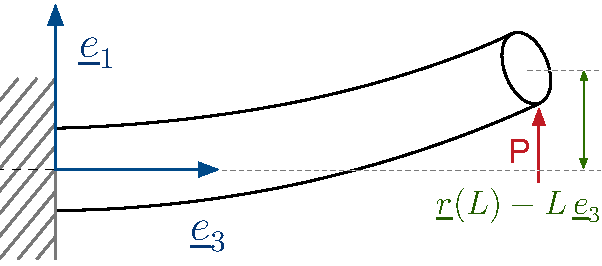
\includegraphics[width=14cm, keepaspectratio=true]{sections/cosserat_rods/images/MinimumPotentialEnergyMethodExample}
  \end{figure}
  
  \vspace{1em}
  we have 12 boundary conditions:
  
  \vspace{0.5em}
  \begin{tabularx}{\linewidth}{XX}
    {
      boundary conditions at $s=0$:
      \begin{itemize}
        \item $\underline{r}(0) = \underline{0}$
        \item $\doubleunderline{R}(0) = \doubleunderline{I} =
          \exp{\doubleunderline{\Theta}} \iff \underline{\Theta}=\underline{0}$
      \end{itemize}
    } & {
      boundary conditions at $s=L$:
      \begin{itemize}
        \item $\doubleunderline{R} \cdot \pd{\psi}{\underline{v}}(L) = P \cdot \underline{e}_1$
        \item $\pd{\psi}{\underline{k}}(L) = \underline{0} \iff M_i = 0 \: (i \in {1,2,3})$
      \end{itemize}
    }
  \end{tabularx}
  
  note that the boundary conditions are not stated in our unknown variables $\underline{v}$, $\underline{k}$
\end{frame}


%-------------------------------------------------------------------------------
\begin{frame}
  \frametitle{Model as a system of first order equations (part 1)}
  
  boundary conditions prescribe not only strains $\left( \underline{v},\underline{k} \right)$,  but also displacements $\left( \underline{r},\doubleunderline{R} \right)$ \newline
  but our model equations depend alone on $\left( \underline{v},\underline{k} \right)$ \newline
  therefore we not yet have a closed system that can be solved \newline
  (by numerically integrating the system of 6 ODEs)
  % TODO BVP: solving the system:
    % 1D problem, no time dependence, only $s$ as independent variable
      % dynamics, inertia term, time derivative, PDE?, FEM  
    % BC on both ends?
    % demands on the solver, Runge-Kutta-scheme
  
  \vspace{0.7em}
  to \textit{close the system}, we will rewrite the model as 12 first order equations, \newline
  by including 6 extra equations relating strain quantities to displacement quantities:
  \begin{displaymath}
    \underline{v} = \doubleunderline{R}^{\mathrm{T}} \cdot \underline{r}^{\prime}
    \Rightarrow
    \underline{r}^{\prime} = \doubleunderline{R} \cdot \underline{v}
  \end{displaymath}
  \begin{displaymath}
    \doubleunderline{K} = \doubleunderline{R}^{\mathrm{T}} \cdot \doubleunderline{R}^{\prime}
    \Rightarrow
    \doubleunderline{R}^{\prime} = \doubleunderline{R} \cdot \doubleunderline{K}
  \end{displaymath}
  
  \vspace{0.7em}
  we already noticed, that using unit quaternions to encode $SO(3)$ matrices has some great advantages for computation. therefore we chose to replace the matrix differential equation in $\doubleunderline{R}$ by a matrix differential equation in terms of unit quaternions $\underline{q} \in \mathbb{R}^4$
  \begin{displaymath}
    \underline{q}^{\prime} = \doubleunderline{E}(\underline{q}) \cdot \underline{k} =
    \frac{1}{2} \cdot \begin{bmatrix}
      -q_1 & -q_2 & -q_3 \\
      +q_0 & -q_3 & +q_2 \\
      +q_3 & +q_0 & -q_1 \\
      -q_2 & +q_1 & +q_0
    \end{bmatrix} \cdot \underline{k}
  \end{displaymath}
\end{frame}

%-------------------------------------------------------------------------------
\begin{frame}
  \frametitle{Model as a system of first order equations (part 2)}

  we have the same 6 equations as before here expressed in matrix form
  
  \begin{displaymath}
    \underbrace{
    \begin{bmatrix}
      \pd[2]{\psi}{\underline{v}} &
      \md{\psi}{2}{\underline{v}}{}{\underline{k}}{} \\
      \md{\psi}{2}{\underline{k}}{}{\underline{v}}{} &
      \pd[2]{\psi}{\underline{k}}
    \end{bmatrix}
    }_{=: \doubleunderline{C}}
    \cdot
    \begin{bmatrix}
      \underline{v}^{\prime} \\
      \underline{k}^{\prime}
    \end{bmatrix} =
    \begin{bmatrix}
      -\underline{k} \times \pd{\psi}{\underline{v}} \\
      -\underline{k} \times \pd{\psi}{\underline{k}}
      -\underline{v} \times \pd{\psi}{\underline{v}}
    \end{bmatrix} -
    \begin{bmatrix}
      \doubleunderline{R}^{\mathrm{T}} \, \underline{\hat{n}} \\
      \doubleunderline{R}^{\mathrm{T}} \, \underline{\hat{m}}
    \end{bmatrix}
  \end{displaymath}
  
  $\doubleunderline{C}$ is the (positive definite) elasticity tensor matrix
  
  \vspace{1em}
  we close the system by adding the seven extra first order equations \newline
  (relating (derivatives of) displacements to strains)
  \begin{displaymath}
    \underline{r}^{\prime} = \doubleunderline{R} \cdot \underline{v}
  \end{displaymath}
  \begin{displaymath}
    \underline{q}^{\prime} = \doubleunderline{E} \cdot \underline{k}
  \end{displaymath}
  
  \vspace{1em}
  $\rightarrow$ this gives us a system of 13 coupled nonlinear ODEs
  
  % TODO write about constraint (7th / 13th equation)
  \begin{displaymath}
    \underline{q} \cdot \underline{q} \overset{!}{=} 1
    \quad \Rightarrow \quad
    \underline{q} \cdot \underline{q}^{\prime} \overset{!}{=} 0
  \end{displaymath}
\end{frame}


%-------------------------------------------------------------------------------
\begin{frame}
  \frametitle{Example with boundary conditions (revisited)}

  \begin{figure}
    \centering
    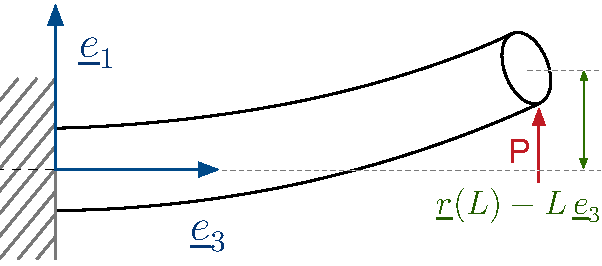
\includegraphics[width=9cm, keepaspectratio=true]{sections/cosserat_rods/images/MinimumPotentialEnergyMethodExample}
  \end{figure}
  
  \vspace{0.7em}
  we have 13 boundary conditions:
  
  \vspace{0.5em}
  \begin{tabularx}{\linewidth}{XX}
    {
      boundary conditions at $s=0$:
      \begin{itemize}
        \item $\underline{r}(0) = \underline{0}$
        \item $\underline{q}(0) =
          \begin{bmatrix}
            1 & 0 & 0 & 0
          \end{bmatrix}^{\mathrm{T}}$ because
          \begin{itemize}
            \item $\: \: \, q_0 = \cos\bigl( \frac{\Theta}{2} \bigr) = 1$ and
            \item $\begin{bmatrix}
            q_1 \\ q_2 \\ q_3
          \end{bmatrix} = \sin \bigl( \frac{\Theta}{2} \bigr) \cdot \underline{a} =
          \begin{bmatrix}
            0 \\ 0 \\ 0
          \end{bmatrix}$
        \end{itemize}
      \end{itemize}
    } & {
      boundary conditions at $s=L$:
      \begin{itemize}
        \item $\doubleunderline{R} \cdot \pd{\psi}{\underline{v}}(L) = P \cdot \underline{e}_1$
        \item $\pd{\psi}{\underline{k}}(L) = \underline{0} \iff$
          \begin{itemize}
            \item $M_i(L) = 0 \: (i \in {1,2,3})$
          \end{itemize}
      \end{itemize}
    }
  \end{tabularx}
\end{frame}


%-------------------------------------------------------------------------------
\begin{frame}
  \frametitle{Another example with boundary conditions: follower load problem}
  % TODO follower load
  \vspace{0.5em}
  \begin{tabularx}{\linewidth}{XX}
    {
      boundary conditions at $s=0$:
      \begin{itemize}
        \item $\underline{r}(0) = \underline{0}$
        \item $\underline{q}(0) =
          \begin{bmatrix}
            1 & 0 & 0 & 0
          \end{bmatrix}^{\mathrm{T}}$ because
          \begin{itemize}
            \item $\: \: \, q_0 = \cos\bigl( \frac{\Theta}{2} \bigr) = 1$ and
            \item $\begin{bmatrix}
            q_1 \\ q_2 \\ q_3
          \end{bmatrix} = \sin \bigl( \frac{\Theta}{2} \bigr) \cdot \underline{a} =
          \begin{bmatrix}
            0 \\ 0 \\ 0
          \end{bmatrix}$
        \end{itemize}
      \end{itemize}
    } & {
      boundary conditions at $s=L$:
      \begin{itemize}
        \item $\doubleunderline{R} \cdot \pd{\psi}{\underline{v}}(L) = P \cdot \underline{d}_1 = \doubleunderline{R} \cdot P \cdot \underline{e}_1 \: \Rightarrow$
          \begin{itemize}
            \item $\pd{\psi}{v_1}(L) = P$
            \item $\pd{\psi}{v_2}(L) = 0$
            \item $\pd{\psi}{v_3}(L) = 0$
          \end{itemize}
        \item $\pd{\psi}{\underline{k}}(L) = \underline{0} \iff$
          \begin{itemize}
            \item $M_i(L) = 0 \: (i \in {1,2,3})$
          \end{itemize}
      \end{itemize}
    }
  \end{tabularx}
\end{frame}


%-------------------------------------------------------------------------------
\begin{frame}
  \frametitle{Yet another example with boundary conditions}
  \vspace{-0.5em}
  \begin{multicols}{2}
    \noindent
    \begin{figure}
      \centering
      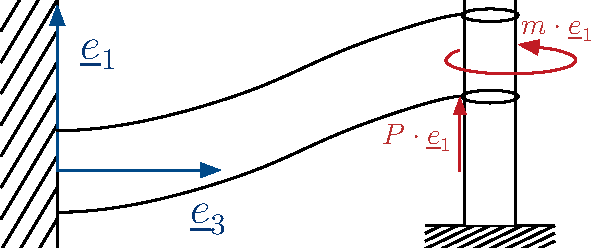
\includegraphics[width=11cm, keepaspectratio=true]{sections/cosserat_rods/images/YetAnotherExampleWithBC}
    \end{figure}
  
    boundary conditions at $s=0$:
    \begin{itemize}
      \item $\underline{r}(0) = \underline{0}$
      \item $\underline{q}(0) =
        \begin{bmatrix}
          1 & 0 & 0 & 0
        \end{bmatrix}^{\mathrm{T}}$ because
        \begin{itemize}
          \item $\: \: \, q_0 = \cos\bigl( \frac{\Theta}{2} \bigr) = 1$ and
          \item $\begin{bmatrix}
          q_1 \\ q_2 \\ q_3
        \end{bmatrix} = \sin \bigl( \frac{\Theta}{2} \bigr) \cdot \underline{a} =
        \begin{bmatrix}
          0 \\ 0 \\ 0
        \end{bmatrix}$
      \end{itemize}
    \end{itemize}
    \vspace{2em}

    boundary conditions at $s=L$:
    \begin{itemize}
      \item $n_1(L) = P$
        \begin{itemize}
          \item $\doubleunderline{R} \cdot \pd{\psi}{\underline{v}}(L) = P \cdot \underline{e}_1 \: \Rightarrow$
          \item $\bigl( \doubleunderline{R} \cdot \pd{\psi}{\underline{v}}(L) \bigr) \cdot \underline{e}_1 = P \: \wedge \: \underline{e}_1 = \underline{d}_1(L) \Rightarrow$
          \item $\pd{\psi}{v_1}(L) = P$
        \end{itemize}
      \item $r_2(L) = 0$
      \item $r_3(L) = L$
      \item $\pd{\psi}{k_1}(L) = m$
      \item $\begin{bmatrix}
              q_1 \\ q_2 \\ q_3
            \end{bmatrix} =
            \sin \bigl( \frac{\Theta}{2} \bigr) \cdot
            \begin{bmatrix}
              1 \\ 0 \\ 0
            \end{bmatrix}
            \: \Rightarrow \: q_2 =0 , \, q_3 = 0$
    \end{itemize}
  \end{multicols}
\end{frame}


%===============================================================================
\subsection{Constitutive laws (part 2)}

%-------------------------------------------------------------------------------
\begin{frame}
  \frametitle{Material symmetry in 3D elasticity}

  \begin{displaymath}
    W \bigl( \doubleunderline{F} \bigr) \overset{\star}{=}
    W \bigl( \doubleunderline{U} \bigr) \overset{\star \star}{=}
    W \bigl( I_1, \, I_2, \, I_3 \bigr)
  \end{displaymath}
  
  \vspace{0.5em}
  \begin{itemize}
    \item $\star$ : principle of frame-indifference
    \item $\doubleunderline{U}$ : ... %TODO U
    \item $\star \star$ : isotropy: material law is the same for all directions in the material %TODO better way to say this?
    \item $I_1$, $I_2$, $I_3$ : strain-invariants
    \item in case of an orthotropic material law, there would simply result a few more invariants ; \newline
      othotropy here means that the material behavior in $s$ direction differs from the behavior in $X_1$, $X_2$ directions
  \end{itemize}
  
  \vspace{1em}
  \textbf{how to obtain the specific form of the energy potential function}? \newline
  remember for example the already postulated function
  % TODO A,C interchanged ; groupby A,C
  \vspace{0.53em}
  \begin{displaymath}
    \psi \bigl( \underline{v}, \, \underline{k} \bigr) =
    \frac{1}{2} \mathscr{A} \, v_1^2 +
    \frac{1}{2} \mathscr{A} \, v_2^2 +
    \frac{1}{2} \mathscr{D} \, (v_3-1)^2 +
    \frac{1}{2} \mathscr{C} \, k_1^2 +
    \frac{1}{2} \mathscr{C} \, k_2^2 +
    \frac{1}{2} \mathscr{B} \, k_3^2
  \end{displaymath}
  
  \vspace{0.3em}
  $\rightarrow$ how to identify the strain invariants? \newline
\end{frame}


%-------------------------------------------------------------------------------
\begin{frame}
  \frametitle{Material symmetry in elastic rods (part 1)}
  
  to get a better understanding of the concept of material symmetry, \newline
  we set up \textbf{another thought experiment}
  \vspace{0.5em}
  \begin{figure}
    \centering
    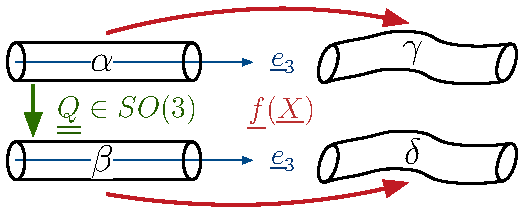
\includegraphics[width=18cm, keepaspectratio=true]{sections/cosserat_rods/images/MaterialSymmetryExperiment}
  \end{figure}
  \begin{itemize}
    \item we start with the reference configuration $\alpha$
    \item we rotate $\alpha$ by $\doubleunderline{Q}$ to get $\beta$ (a rotated reference configuration)
    \item $\underline{f}(.)$ maps $\alpha \mapsto \gamma$ and $\beta \mapsto \delta$
  \end{itemize}
  
  if $\doubleunderline{Q}$ is in the symmetry group $\mathscr{G}$ then then we have $\eval[1]{\psi}_{\gamma} = \eval[1]{\psi}_{\delta}$
\end{frame}


%-------------------------------------------------------------------------------
\begin{frame}
  \frametitle{Material symmetry in elastic rods (part 2)}

  \begin{enumerate}
    \item configuration $\gamma$ (image of reference configuration $\alpha$)
      \begin{itemize}
        \item $\underline{r}^{\gamma}(s)$
        \item $\doubleunderline{R}^{\gamma}(s)$
      \end{itemize}
    \item configuration $\delta$ (image of rotated reference configuration $\beta$)
      \begin{itemize}
        \item $\underline{r}^{\delta}(s) =
                \underline{r}^{\gamma}(s)$
        \item $\doubleunderline{R}^{\delta}(s) =
                \doubleunderline{R}^{\gamma}(s) \cdot \doubleunderline{Q}$
        \item $\underline{v}^{\delta}(s) =
                \doubleunderline{R}^{\gamma \mathrm{T}}(s) \cdot \underline{r}^{\gamma \prime}(s) =
                \doubleunderline{Q}^{\mathrm{T}} \cdot \doubleunderline{R}^{\gamma \mathrm{T}}(s) \cdot \underline{r}^{\gamma \prime}(s) =
                \doubleunderline{Q}^{\mathrm{T}} \cdot \underline{v}^{\gamma}(s)$
        \item $\underline{k}^{\delta} =
                \axial \bigl( \doubleunderline{R}^{\delta \mathrm{T}} \cdot \doubleunderline{R}^{\delta \prime} \bigr) =
                \axial \bigl( \doubleunderline{Q}^{\mathrm{T}} \cdot \doubleunderline{R}^{\gamma \mathrm{T}} \cdot \doubleunderline{R}^{\gamma \prime} \cdot \doubleunderline{Q} \bigr) =
                \doubleunderline{Q}^{\mathrm{T}} \cdot \axial \bigl( \doubleunderline{R}^{\gamma \mathrm{T}} \cdot \doubleunderline{R}^{\gamma \prime} \bigr) =
                \doubleunderline{Q}^{\mathrm{T}} \cdot \underline{k}^{\gamma}$
      \end{itemize}
  \end{enumerate}
  
  \begin{displaymath}
    \Rightarrow
    \psi \bigl( \doubleunderline{Q}^{\mathrm{T}} \cdot \underline{v}^{\gamma}, \, \doubleunderline{Q}^{\mathrm{T}} \cdot \underline{k}^{\gamma} \bigr) \overset{!}{=}
    \psi \bigl( \underline{v}^{\gamma}, \, \underline{k}^{\gamma} \bigr)
    \: \forall \doubleunderline{Q} \in \mathscr{G}
  \end{displaymath}
  
  \vspace{0.5em}
  \begin{itemize}
    \item the symmetry group $\mathscr{G}$ depends on geometry and on the material of the beam
    \item $\mathscr{G} \equiv SO(2)$ (all rotations about $\underline{e}_3$-axis), if beam has circular cross section and isotropic material ; also the case for circular ropes with continuous helicity
  \end{itemize}
  
\end{frame}


%-------------------------------------------------------------------------------
\begin{frame}
  \frametitle{Material symmetry in elastic rods (part 3)}
  \vspace{-0.4em}
  with $\mathscr{G} \equiv SO(2)$ we had ...
  \begin{displaymath}
    \doubleunderline{Q} =
    \begin{bmatrix}
      +\cos(\Theta) & -\sin(\Theta) & 0 \\
      +\sin(\Theta) & +\cos(\Theta) & 0 \\
      0 & 0 & 1
    \end{bmatrix}
    \quad \forall \: \Theta \in [0,2\,\pi]
  \end{displaymath}
  \begin{displaymath}
    \underline{v}^{\delta} =
    \doubleunderline{Q}^{\mathrm{T}} \cdot \underline{v}^{\gamma} =
    \begin{bmatrix}
      \begin{bmatrix}
        +\cos(\Theta) & +\sin(\Theta) \\
        -\sin(\Theta) & +\cos(\Theta)
      \end{bmatrix} \cdot
      \begin{bmatrix}
        v_1^{\gamma} \\ v_2^{\gamma}
      \end{bmatrix} \\
      v_3^{\gamma}
    \end{bmatrix}
    \: ; \quad
    \underline{v}^{\delta} = \dots \text{(replace }v\text{ by }k\text{)}
  \end{displaymath}
  we introduce some abbreviations ...
  \begin{displaymath}
    \underline{v}^{\delta} =
    \begin{bmatrix}
      \doubleunderline{\hat{Q}}^{\mathrm{T}} \cdot \underline{\hat{v}}^{\gamma} \\
      v_3^{\gamma}
    \end{bmatrix}   
    \text{ with }
    \underline{\hat{v}}^{\gamma} =
    \begin{bmatrix}
      v_1^{\gamma} \\ v_2^{\gamma}
    \end{bmatrix}
    \text{ and }
    \doubleunderline{\hat{Q}} =
    \begin{bmatrix}
      +\cos(\Theta) & -\sin(\Theta) \\
      +\sin(\Theta) & +\cos(\Theta)
    \end{bmatrix}
  \end{displaymath}
  
  \vspace{0.4em}
  we observe the following \textbf{invariants} under all such transformations $\doubleunderline{Q} \in \mathscr{G}$
  \begin{itemize}
    \item angle between and magnitude of $\underline{\hat{v}}$, $\underline{\hat{k}}$
      $\quad \rightarrow \quad$
      $\enVert[1]{\underline{\hat{v}}}$ , $\enVert[1]{\underline{\hat{k}}}$ , $\underline{\hat{v}} \cdot \underline{\hat{k}}$ , $\left( \underline{\hat{v}} \times \underline{\hat{k}} \right) \cdot \underline{e}_3$
    \item $v_3$, $k_3$
  \end{itemize}
  
  \vspace{-1em}
  \begin{displaymath}
    \Rightarrow
    \psi = \psi \bigl(
      \underbrace{v_1^2 + v_2^2}_{I_1} , \, \underbrace{k_1^2 + k_2^2}_{I_2} , \, \underbrace{v_1 \cdot k_1 + v_2 \cdot k_2}_{I_3} , \, \underbrace{v_1 \cdot k_2 - v_2 \cdot k_1}_{I_4} , \, \underbrace{v_3}_{I_5} , \, \underbrace{k_3}_{I_6}
    \bigr)
  \end{displaymath}
\end{frame}

%-------------------------------------------------------------------------------
\begin{frame}
  \frametitle{Material symmetry in elastic rods (part 4)}
  \vspace{-1em}
  \begin{displaymath}
    \psi = \psi \bigl(
      \underbrace{v_1^2 + v_2^2}_{I_1} , \, \underbrace{k_1^2 + k_2^2}_{I_2} , \, \underbrace{v_1 \cdot k_1 + v_2 \cdot k_2}_{I_3} , \, \underbrace{v_1 \cdot k_2 - v_2 \cdot k_1}_{I_4} , \, \underbrace{v_3}_{I_5} , \, \underbrace{k_3}_{I_6}
    \bigr)
  \end{displaymath}

  \vspace{0.5em}
  as \textbf{another experiment} consider now a reflection of the beam about the $\underline{e}_1$-$\underline{e}_2$-plane
  
  \vspace{0.3em}
  $\rightarrow$ such a transformation is not in the symmetry group for a pre-twisted rod
  
  \vspace{0.3em}
  $\rightarrow$ $I_4$, $I_5$, $I_6$ will change their sign
  
  \vspace{0.5em}
  we do a Taylor-expansion of $\psi$ about $\bigl( \underline{v}_0 , \, \underline{k}_0 \bigr) = \bigl( \begin{bmatrix}
    0 & 0 & 1
  \end{bmatrix}^{\mathrm{T}} , \, \begin{bmatrix}
    0 & 0 & 0
  \end{bmatrix}^{\mathrm{T}} \bigr)$
  \begin{displaymath}
    \psi \bigl( \underline{v}, \, \underline{k} \bigr) =
    \cancel{ \psi \bigl( \underline{v}_0, \, \underline{k}_0 \bigr) } +
    \cancel{ \pd{\psi}{\underline{v}} \bigl( \underline{v}_0, \, \underline{k}_0 \bigr) \cdot \bigl( \underline{v} - \underline{v}_0 \bigr) } +
    \cancel{ \pd{\psi}{\underline{k}} \bigl( \underline{v}_0, \, \underline{k}_0 \bigr) \cdot \bigl( \underline{k} - \underline{k}_0 \bigr) } +
  \end{displaymath}
  \begin{displaymath}
    + \frac{1}{2} \Biggl(
      \Bigl( \pd[2]{\psi}{\underline{v}} \cdot \bigl( \underline{v} - \underline{v}_0 \bigr) \Bigr) \cdot \bigl( \underline{v} - \underline{v}_0 \bigr) + 
      \Bigl( \pd[2]{\psi}{\underline{k}} \cdot \bigl( \underline{k} - \underline{k}_0 \bigr) \Bigr) \cdot \bigl( \underline{k} - \underline{k}_0 \bigr) +
  \end{displaymath}
  \begin{displaymath}
      + 2 \cdot \Bigl( \md{\psi}{2}{\underline{v}}{}{\underline{k}}{} \cdot \bigl( \underline{k} - \underline{k}_0 \bigr) \Bigr) \cdot \bigl( \underline{v} - \underline{v}_0 \bigr)
    \Biggr) + \text{higher order terms}
  \end{displaymath}
  
  \begin{itemize}
    \item first term has been canceled because it is a constant (irrelevant for potential)
    \item second and third term have been canceled because they depend on the sign % TODO correct? ; 2 \cdot in Taylor in mixed term
  \end{itemize}
\end{frame}


%-------------------------------------------------------------------------------
\begin{frame}
  \frametitle{Material symmetry in elastic rods (part 5)}

  from the Taylor expansion of $\psi$ consider for example the term
  \begin{displaymath}
    \pd[2]{\psi}{\underline{v}} =
    \pd{}{\underline{v}} \biggl( \pd{\psi}{\underline{v}} \biggr) =
    \pd{}{\underline{v}} \biggl( \pd{\psi}{I_1} \cdot \pd{I_1}{\underline{v}} + \dots + \pd{\psi}{I_6} \cdot \pd{I_6}{\underline{v}} \biggr) = \dots
  \end{displaymath}
  
  $\pd{\psi}{I_j}$ are unknowns ($\mathscr{A}, \mathscr{B}, \dots$) that must be obtained from kinematics and 3D elasticity, \newline %TODO more precisely
  whereas $\pd{I_j}{\underline{v}}$ can be computed easily ($j = 1,\dots,6$)
  
  \vspace{1em}
  doing the computations and collecting unknown the coefficients ($\mathscr{A}, \mathscr{B}, \dots$) we obtain
  \begin{displaymath}
    \psi =
    \frac{1}{2} \Bigl(
      \mathscr{A} \cdot \bigl( k_1^2 + k_2^2 \bigr) +
      \mathscr{B} \cdot k_3^2 +
      \mathscr{C} \cdot \bigl( v_1^2 + v_2^2 \bigr) +
      \mathscr{D} \cdot \bigl( k_3 - 1 \bigr)^2 +
  \end{displaymath}
  \begin{displaymath}
    + 2 \cdot \mathscr{E} \cdot \bigl( v_3 - 1 \bigr) \cdot k_3 +
      2 \cdot \mathscr{F} \cdot \bigl( v_1 \cdot k_1 + v_2 \cdot k_2 \bigr)
    \Bigr)
  \end{displaymath}
  %TODO A,C interchanged ; groupby A,C
  
\end{frame}
  




%-------------------------------------------------------------------------------
% include section ...
%\include{sections/blueprint/blueprint}



%-------------------------------------------------------------------------------
\end{document}
